\section{Results} \label{sec:results}


\subsection{PTC}

As part of this project, an initial and fundamental task was to use the PTC to determine the essential parameters of each CCD segment across the focal plane, using the \textit{DM stack}. This has already been done by SLAC National Acceleration Laboratory \footnote{El código utilizado por \textit{SLAC} está disponible en \href{https://github.com/lsst-camera-dh/eotest/blob/32c17b0a33b9c099651ed581ee90c1b1101012fb/python/lsst/eotest/sensor/ptcTask.py}{SLAC code}} (hereafter SLAC) for this very run (\href{https://srs.slac.stanford.edu/BOT_EO_Reports/13144/}{SLAC heat maps BOT 13144}) and here we seek to reproduce their results.



\vspace{3mm}

%%%%%%%%%%%%Figura

\begin{figure}[!htb]
    \centering
    \includegraphics[width=\textwidth]{Figures/PTC_Detector55.png}
    \caption{PTC for all segments of sensor 55 (E2V). Xs represent the data, the red line is the fit to the PTC by exponential approximation (eq. \ref{eq:Astier16}), and the green line is a linear fit. The parameters obtained from the fit to the PTC are the gain, the $a_{00}$ parameter, the PTC turnoff (Max ADU), and the read noise. }
    \label{fig:PTC_55}
\end{figure}

%%%%%%%%%%%%%%%%%%

Initially, we generated the PTCs by CCD for the entire focal plane, as shown in Figure \ref{fig:PTC_55}, to detect PTCs with abnormal behavior and low PTC-turnoff (below 40000 ADU). Detectors found with low PTC-turnoff and/or misclassified are recorded in the table \ref{tab:PTC_warnings}. In addition, a visual inspection showed that about 60 \% of the detectors have at least one segment showing \textit{Downing dip}. 

\vspace{3mm}
%%%%%%%%%%%%Figura

\begin{figure}[!htb]
 \centering
     \begin{subfigure}[b]{0.49\textwidth}
         \centering
         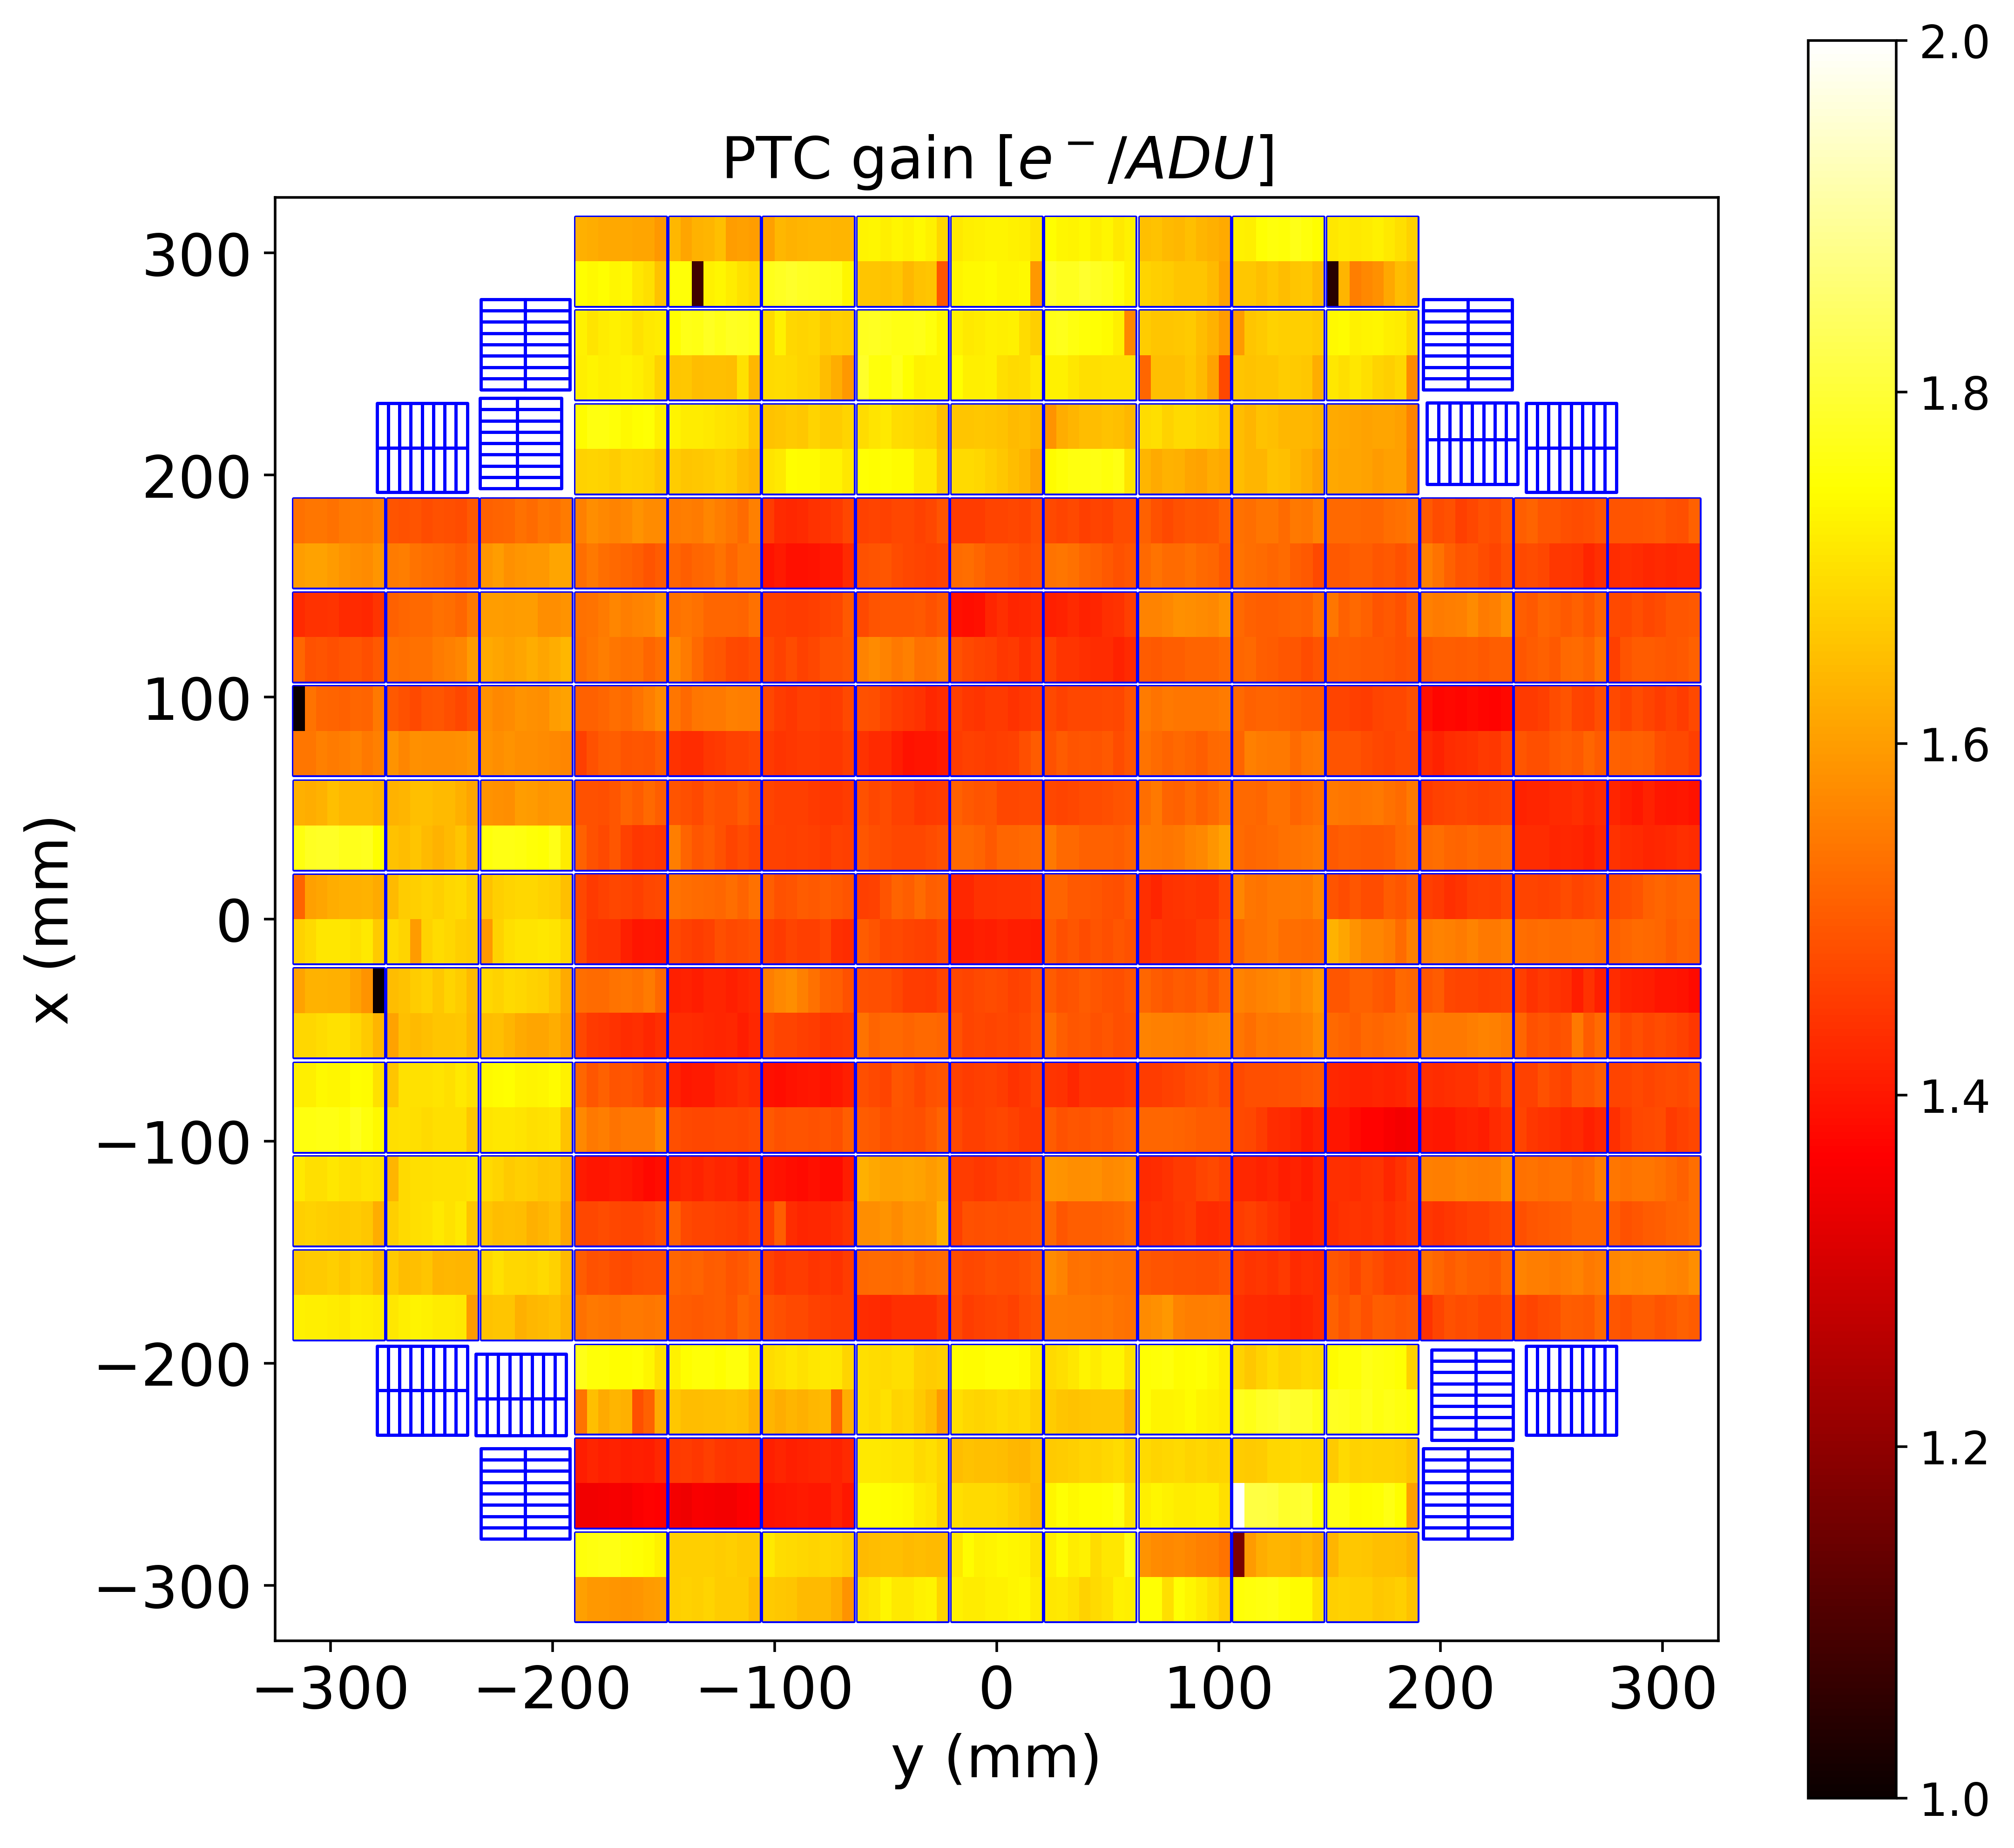
\includegraphics[width=\textwidth]{Figures/Focal_plane_gain.png}
     \end{subfigure}
     \hfill %\hspace{-10em}
     \begin{subfigure}[b]{0.49\textwidth}
         \centering
         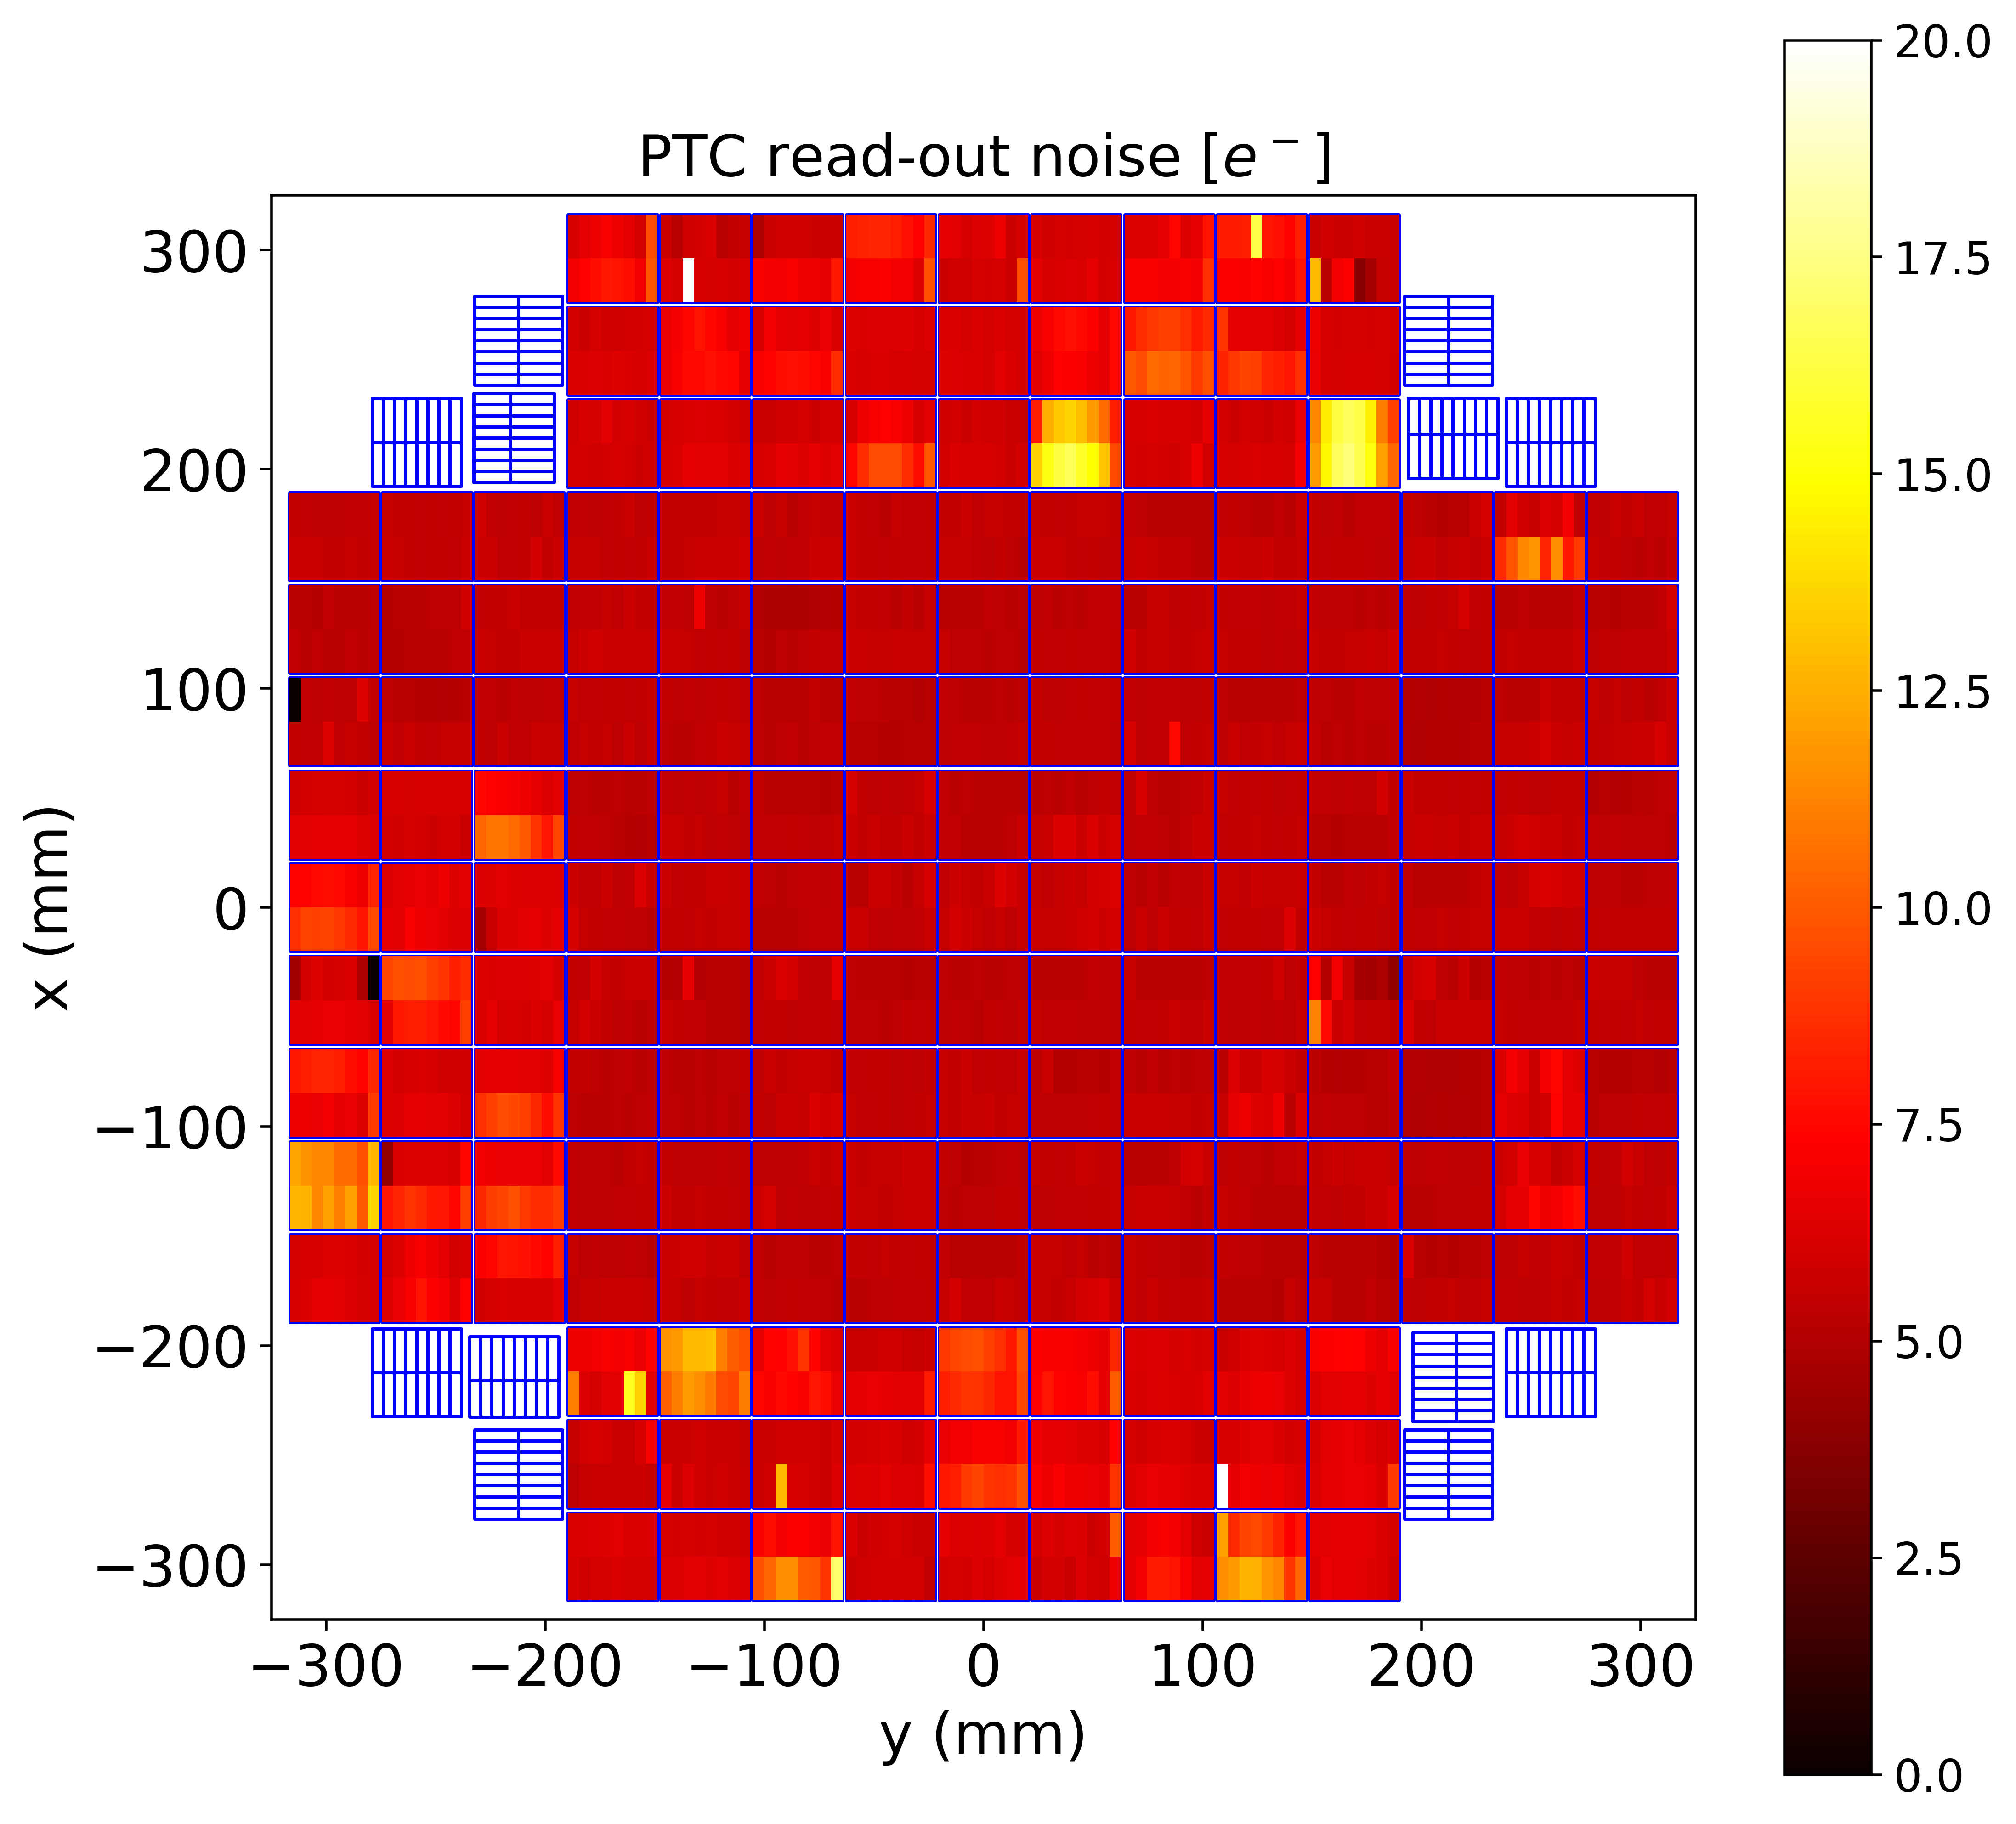
\includegraphics[width=\textwidth]{Figures/Focal_plane_noise.png}
     \end{subfigure}
     \vspace{3mm}
     \begin{subfigure}[b]{0.49\textwidth}
         \centering
         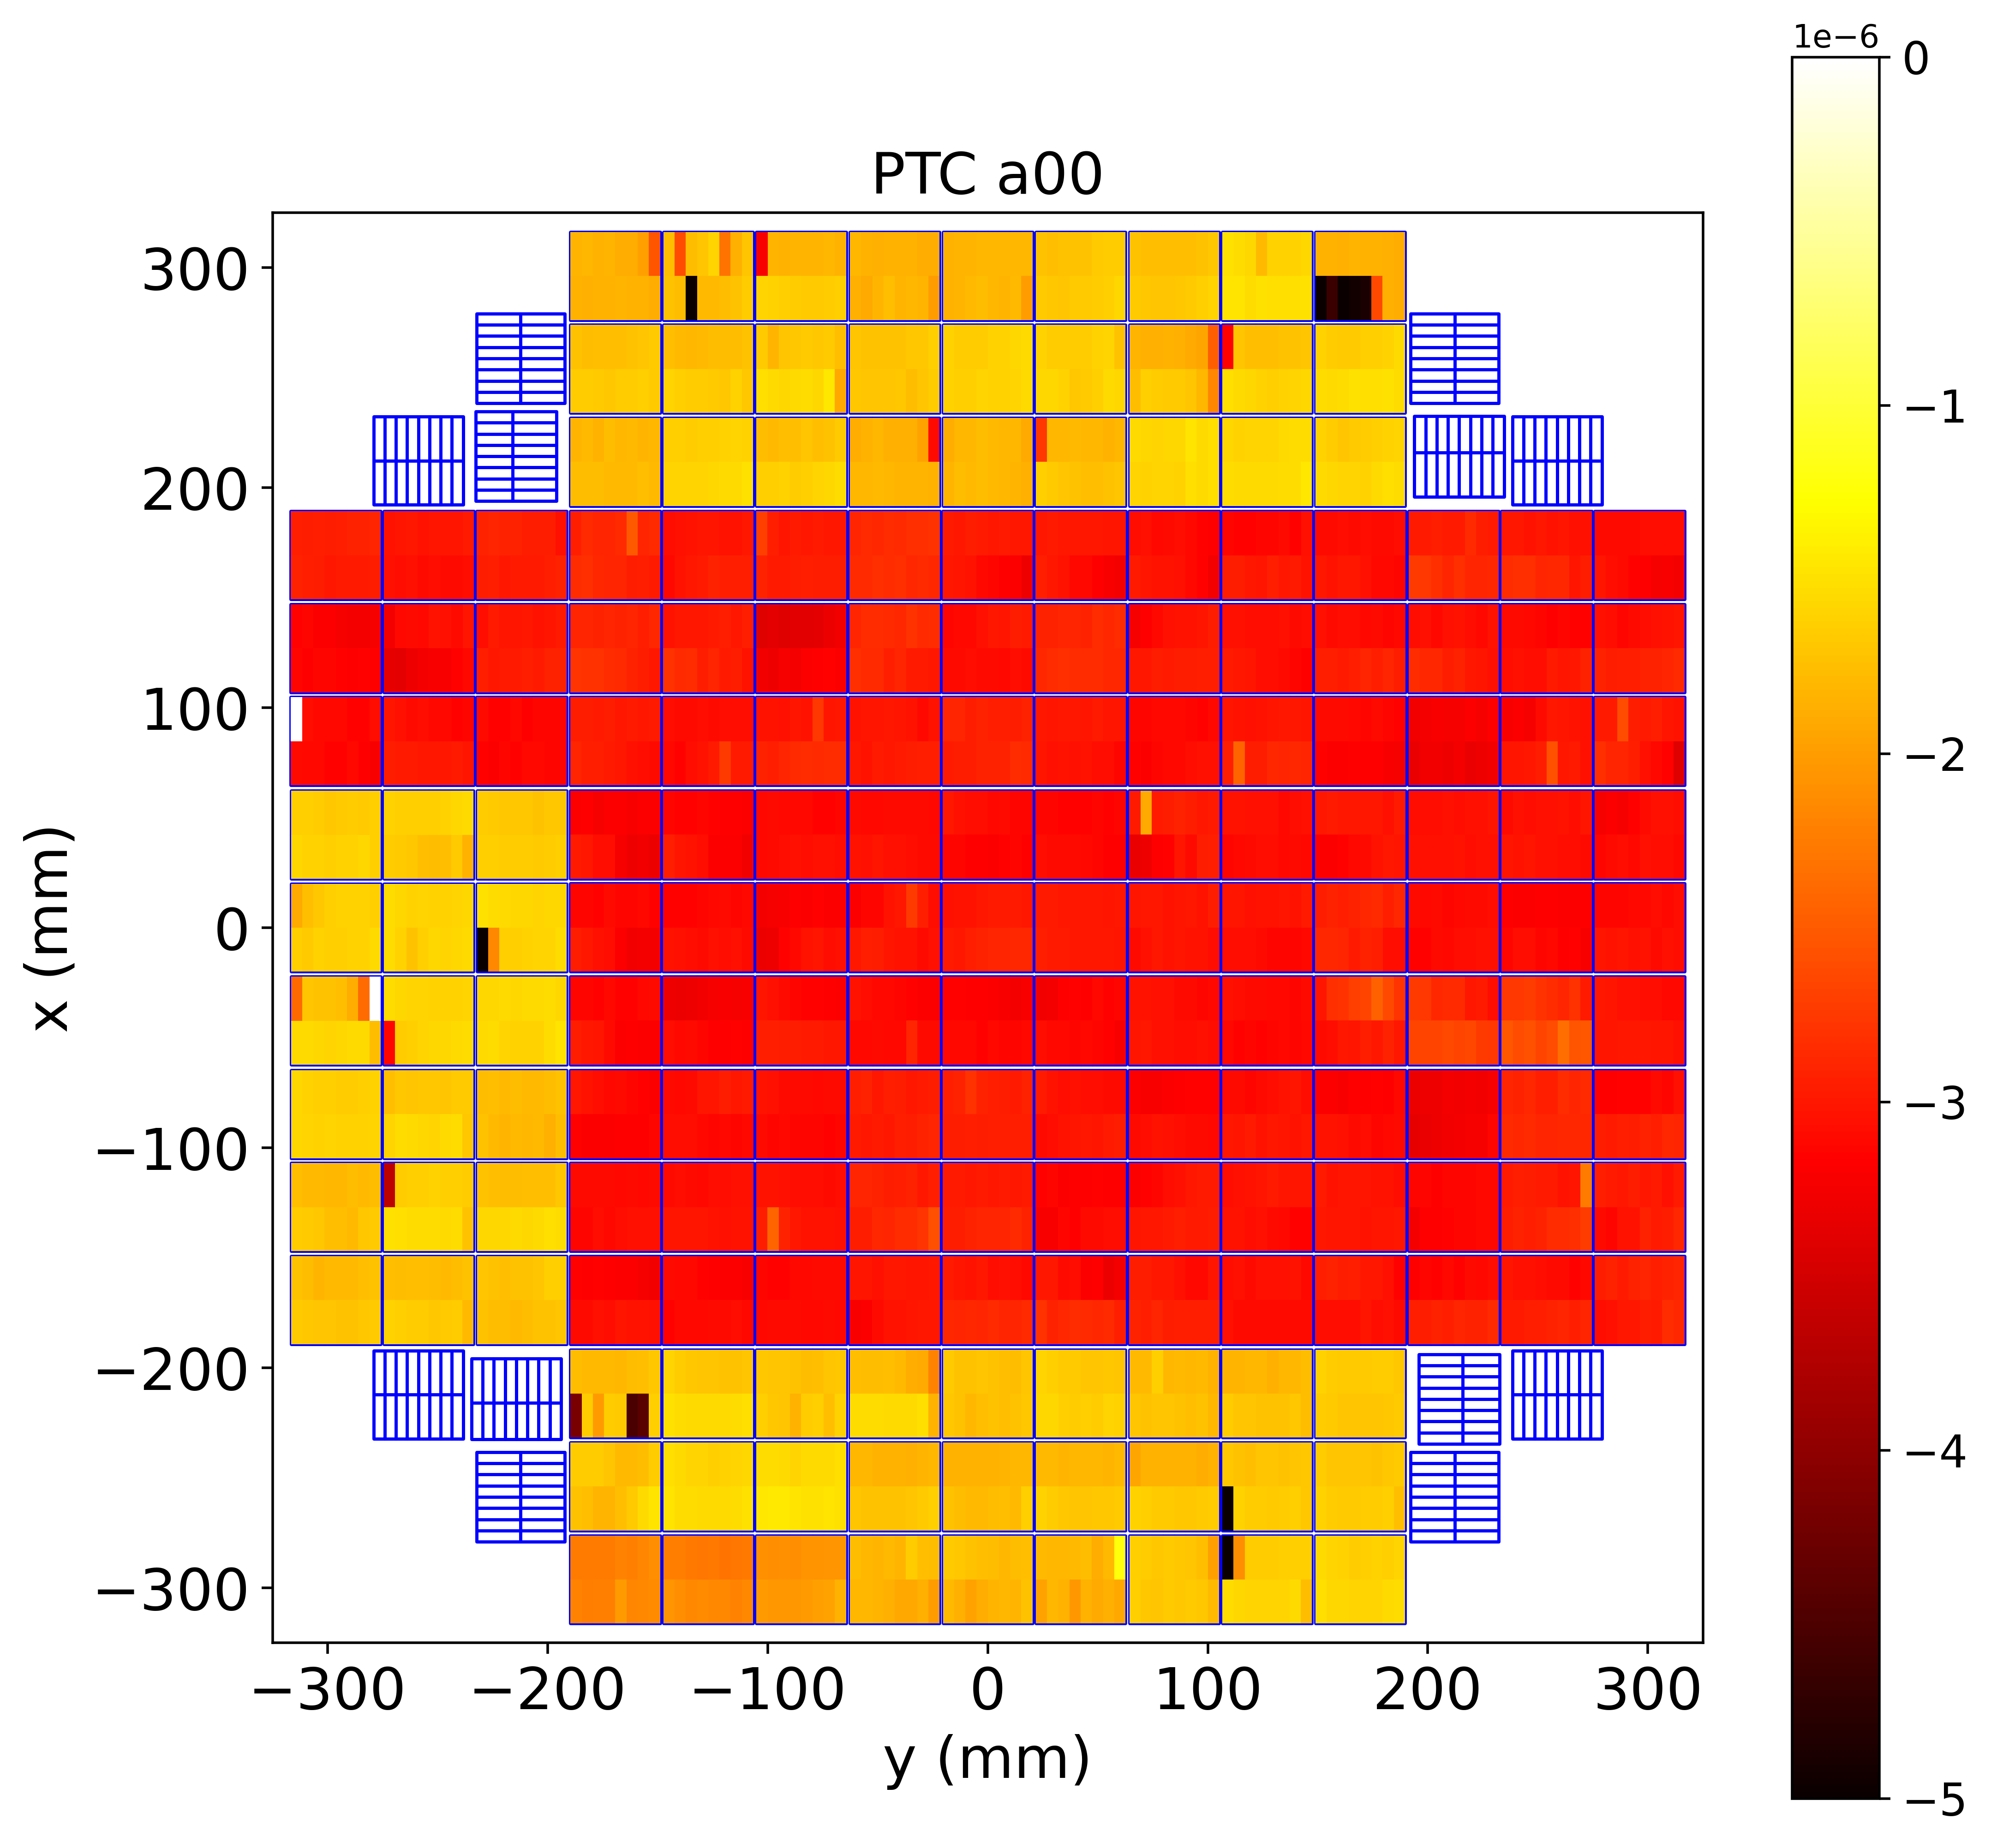
\includegraphics[width=\textwidth]{Figures/Focal_plane_a00.png}
     \end{subfigure}    
     \hfill
     \begin{subfigure}[b]{0.49\textwidth}
         \centering
         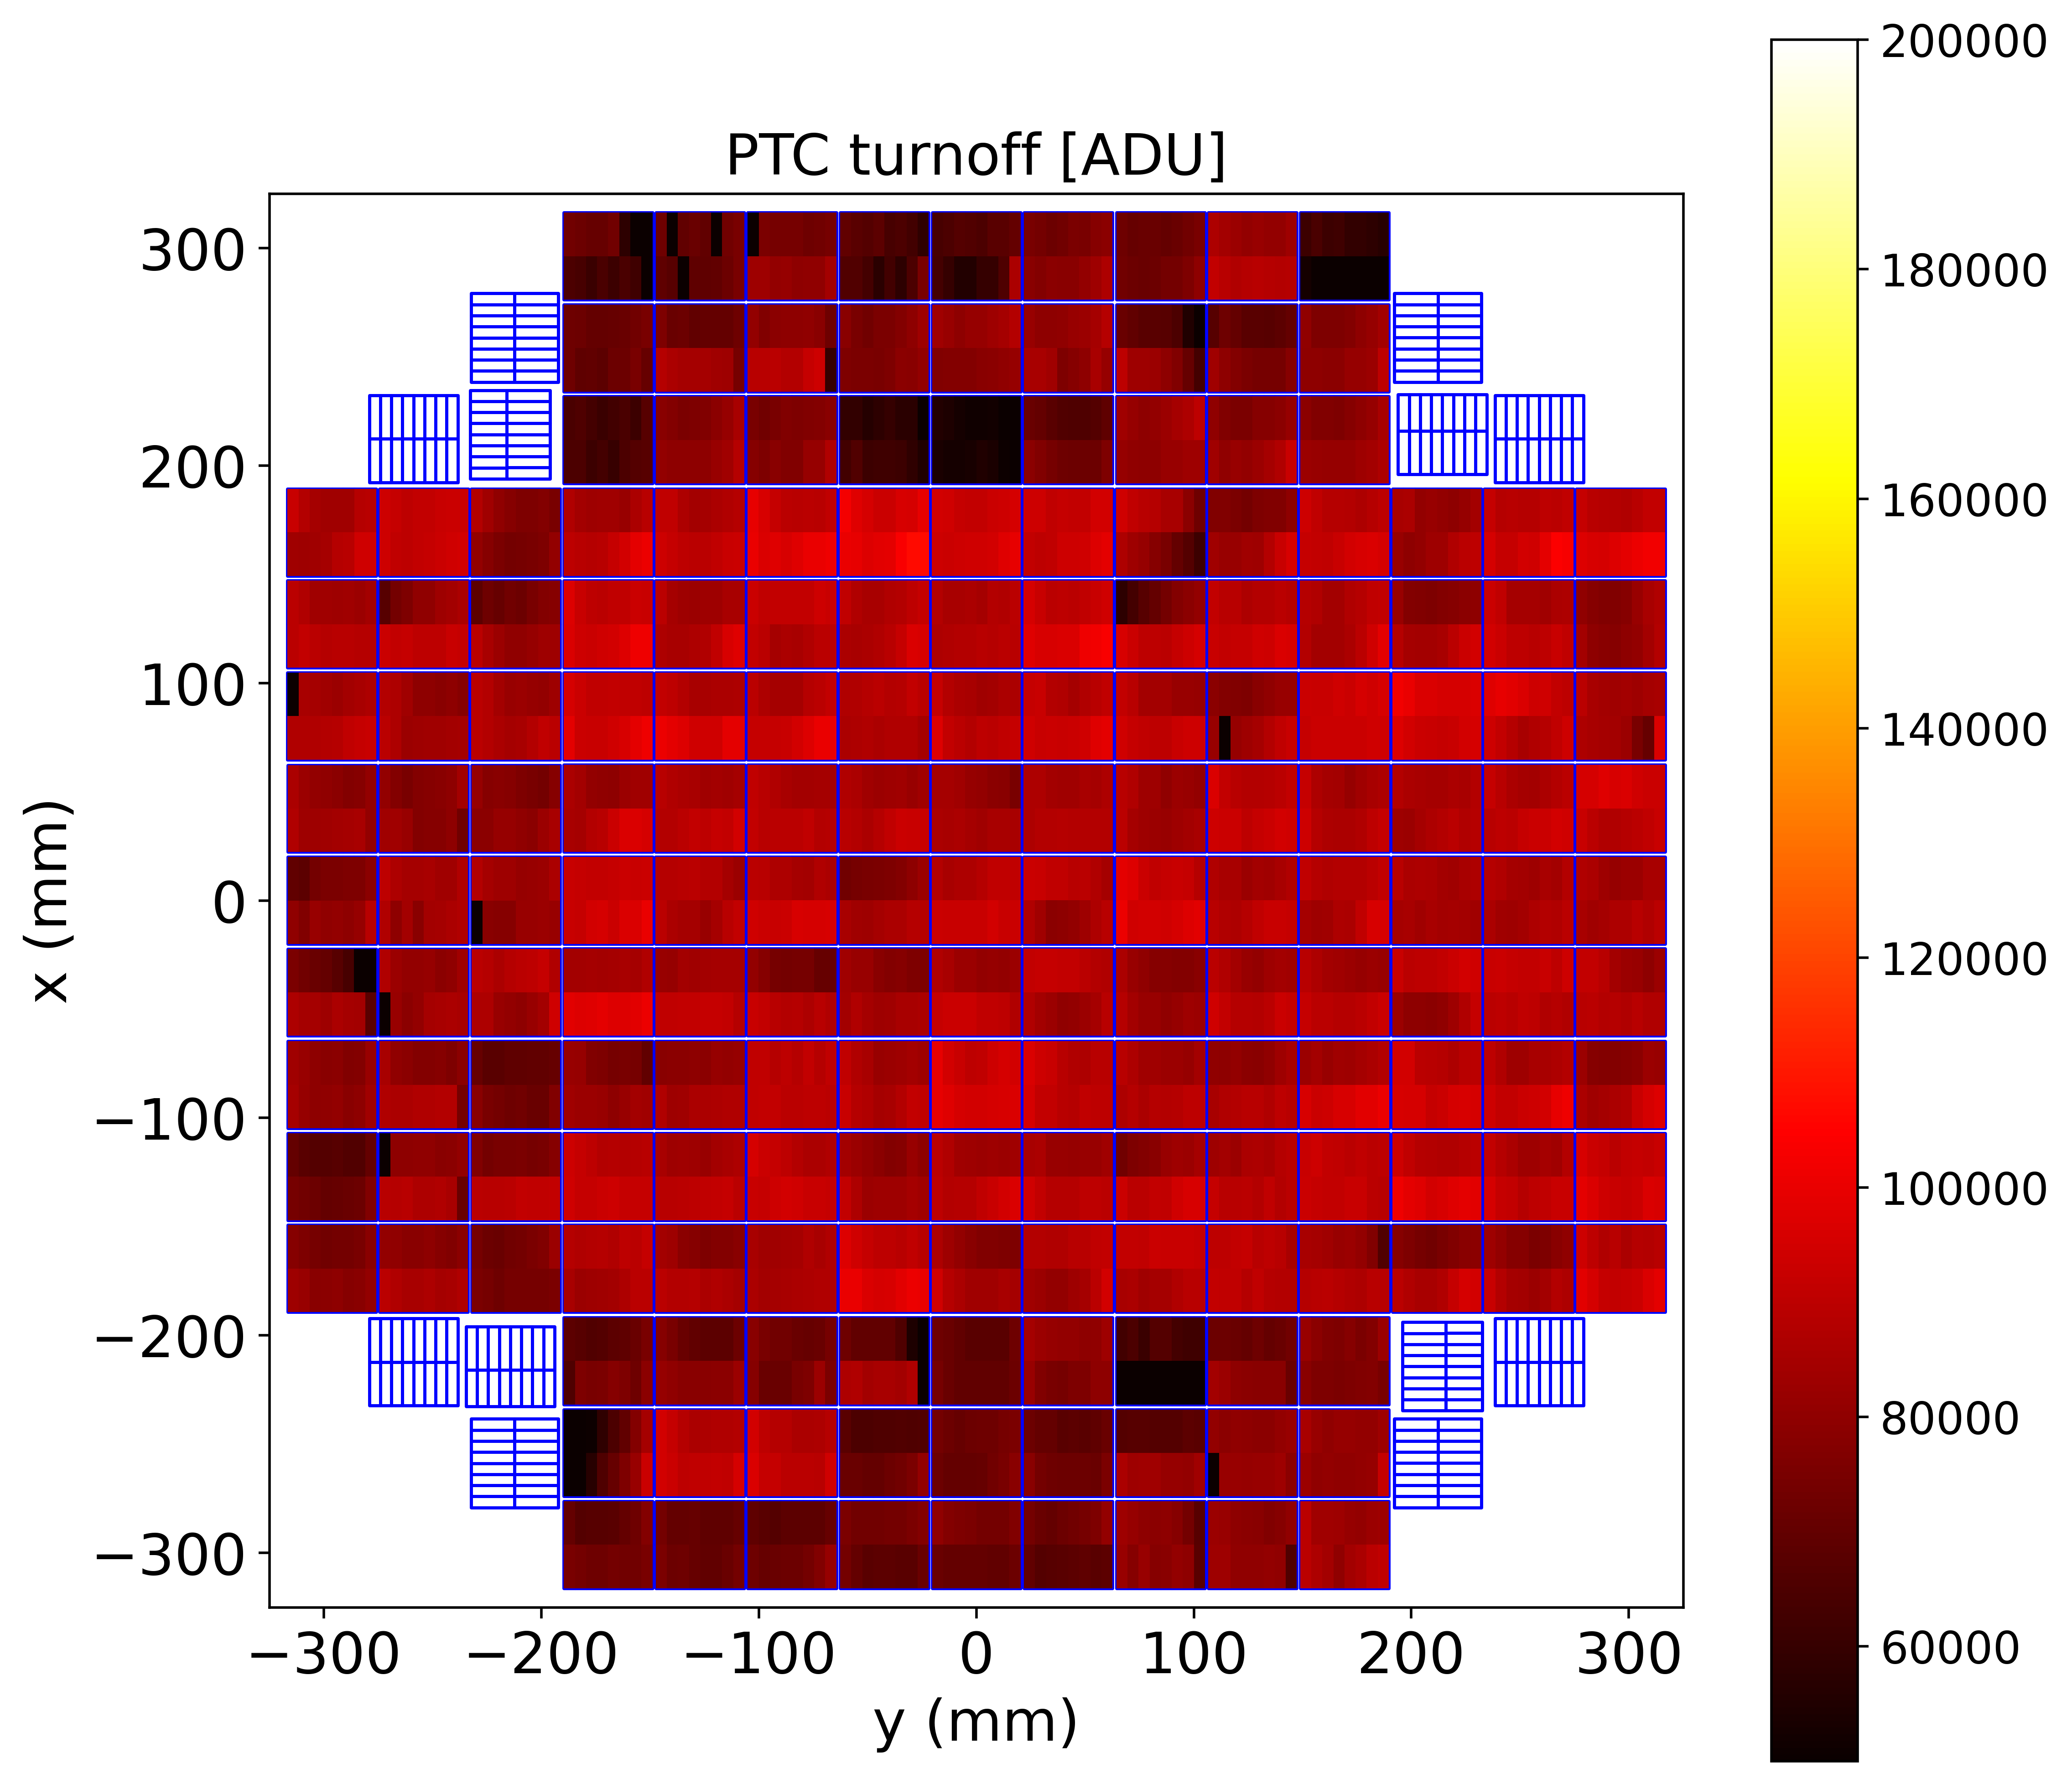
\includegraphics[width=\textwidth]{Figures/Focal_plane_turnoff.png}
     \end{subfigure}
        \caption{Heatmaps for the entire focal plane of the parameters obtained by the fit to the PTC in each segment that makes up the sensors. The upper panel shows the gain values on the left and the read noise on the right. The lower panel shows on the left the values of $a_{00}$, which are of the order of $-1 \times 10 ^{-6}$, and on the right, the turnoff. These maps are a reproduction of those already constructed by SLAC for this same run 13144 (\href{https://srs.slac.stanford.edu/BOT_EO_Reports/13144/}{SLAC heat maps}).}
        \label{fig:FocalPlane_PTC}
\end{figure}
%%%%%%%%%%%%%%%%%%

Subsequently, we generate heat maps for the entire focal plane similar to those performed by SLAC, shown in the panels of Figure \ref{fig:FocalPlane_PTC}, for the parameters estimated by the fit to the PTC: gain and read noise in the upper left and right panel, respectively; $a_{00}$ and turnoff in the lower left and right panel, respectively. A bimodality is found in the gain and $a_{00}$ value (which accounts for the B-F effect); the more reddish values dominate in the E2V sensors, while the more yellow values dominate in ITL; this means that the E2V vendor's detectors have in general a lower gain, but a more negative B-F effect coefficient concerning ITL. Whereas, for readout noise and turnoff, no relevant effect is exhibited due to the vendor. 

\vspace{3mm}

El comportamiento descrito anteriormente por los mapas de calor son reforzados por los histogramas de la figura \ref{fig:Histogram_PTC}, los cuales revelan la clara bimodalidad para la ganancia y $a_{00}$ y un comportamiento más generalizado para el ruido de lectura y el turnoff. La ganancia tiene un valor promedio para los sensores de E2V de $1.49 \pm 0.05$ y de $1.69 \pm 0.05$ $e^{-}/ADU$ para ITL. El coeficiente del B-F effect tiene un valor medio de $(-3.0 \pm 0.1)\times 10 ^{-6}$  y $(-1.7 \pm 0.2)\times 10 ^{-6}$ para E2V e ITL, respectivamente.

The histograms support the behavior described above by the heat maps in Figure \ref{fig:Histogram_PTC}, which reveal clear bimodality for gain and $a_{00}$ and more generalized behavior for read noise and turnoff. The gain has an average value for the E2V sensors of $1.49 \pm 0.05$ and $1.69 \pm 0.05$ $e^{-}/ADU$ for ITL. The BF effect coefficient has an average value of $(-3.0 \pm 0.1)\times 10 ^{-6}$ and $(-1.7 \pm 0.2)\times 10 ^{-6}$ for E2V and ITL, respectively.

\vspace{3mm}

%%%%%%%%%%%%Figura
\begin{figure}[!htb]
    \centering
    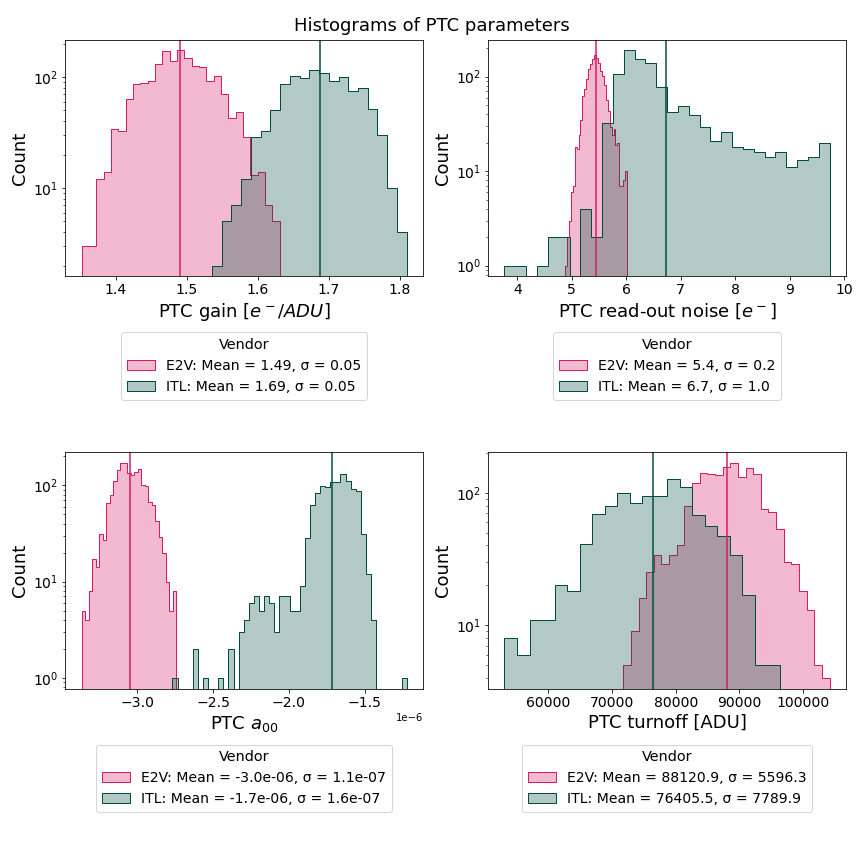
\includegraphics[width=\textwidth]{Figures/Histograms_PTC.png}
    \caption{Histograms for the parameters obtained from the fit to the PTC: gain (top left), read noise (top right), $a_{00}$ (bottom left), and turnoff (bottom right), each of the distributions are shown by vendor, in magenta for E2V and blue for ITL. The vertical lines represent the mean of each distribution. }
    \label{fig:Histogram_PTC}
\end{figure}

%%%%%%%%%%%%%%%%%%

Although, in general, the results between this work and SLAC are congruent, we find differences in some segments for gain, especially in segments C04 and C14 of detector 0 (R01\_S00), C00 of detector 22 (R03\_S11) and C02 of detector 169 (R41\_S21). In table \ref{tab:PTC_warnings} we report in red the segments where we found the most notorious difference between our and the SLAC results for the four parameters (gain, BF coefficient, read noise, and turnoff). For the segments mentioned above, the table shows that detector 22 is possibly dead; in contrast, for the segment of detector 169, there is a misclassification by the PTC-turnoff location algorithm. For these particular segments, the before mentioned can be the reason for the difference between SLAC and us. However, to determine which is causing the differences precisely, it is necessary to conduct a detailed analysis of the respective codes used and their versions. Differences between the algorithms may lead to these differences because we used the same run (13144). It can be differences in the pixels used for the calculation due to the masks used, differences in the reduction of the images (Instrument Signature Removal or ISR), or different rejection of outliers, among others. 


\vspace{3mm}

%%%%%%%%%%%%Figura

\begin{figure}[!htb]
%\raggedleft
     \begin{subfigure}[b]{\textwidth}
         
         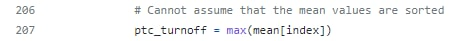
\includegraphics[width=0.7\textwidth,left]{Figures/eotest_turnoff.jpg}
         \caption{Eotest code}
     \end{subfigure}
     \vspace{3mm}
     \begin{subfigure}[b]{\textwidth}
         
         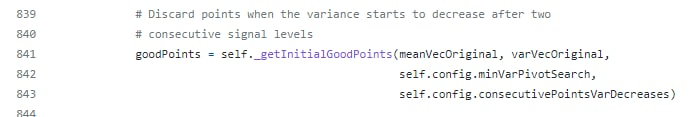
\includegraphics[width=\textwidth,left]{Figures/DMstack_turnoff1.jpg}
     \end{subfigure}    
     \vspace{3mm}
     \begin{subfigure}[b]{\textwidth}
         
         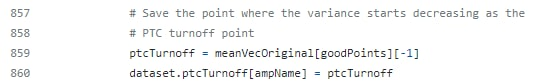
\includegraphics[width=0.85\textwidth,left]{Figures/DMstack_turnoff2.jpg}
         \caption{DM stack code}
     \end{subfigure}
        \caption{Codes used to calculate the PTC-turnoff in \href{https://github.com/lsst-camera-dh/eotest/blob/32c17b0a33b9c099651ed581ee90c1b1101012fb/python/lsst/eotest/sensor/ptcTask.py}{eotest}  (a), used by SLAC, and \href{https://github.com/lsst/cp_pipe/blob/6bae47012f2f119b186509ce7efd963b68b61f0d/python/lsst/cp/pipe/ptc/cpSolvePtcTask.py}{DM stack} (b), official code for LSST data.}
        %Códigos utilizados para calcular el PTC-turnoff en \href{https://github.com/lsst-camera-dh/eotest/blob/32c17b0a33b9c099651ed581ee90c1b1101012fb/python/lsst/eotest/sensor/ptcTask.py}{eotest} (a), empleado por SLAC, y \href{https://github.com/lsst/cp_pipe/blob/6bae47012f2f119b186509ce7efd963b68b61f0d/python/lsst/cp/pipe/ptc/cpSolvePtcTask.py}{DM stack} (b), código oficial para los datos del LSST.}
        \label{fig:Turnoff_codes}
\end{figure}
%%%%%%%%%%%%%%%%%%


For the turn-off, we generally observed similar behavior for the sensors between this work and SLAC. However, the way of determination used different methods, as shown in figure \ref{fig:Turnoff_codes}. On the one hand, \textit{eotest} defines the PTC-turnoff as the point where the variance is maximum, where the maximum value is determined among the data whose residuals are below $5sigma$. In contrast, \textit{DM stack} defines this as the point where the variance starts to decrease monotonically by at least two points (the number of points to decrease can be modified in the function \_getInitialGoodPoints). By SLAC, the FWC found was $\sim 90000$ e$^-$ \colorbox{red}{referencia?}. In contrast, in this work, we found an average value of turnoff with a value of $83240$ ADU, whose equivalence in electrons would be an approximate value of the FWC of $130000 \pm 10000$ e$^-$.

\begin{landscape}
\begin{table}[!htb]
\centering
\caption{Detectors containing segments with low PTC-turnoff (below 40000 ADU), PTC-turnoff misclassified by the algorithm, bad segments, or differences observed concerning the results obtained by SLAC (parameters in red). Presented for each segment is the detector ID (col1), detector number (col2), vendor (col3), affected segment (col4), PTC parameters (gain, B-F effect, and turnoff coefficient; cols 5, 6, 7, and 8, respectively), detected problem (col9).}
\label{tab:PTC_warnings}
\begin{tabular}{ccccccccp{0.2\textwidth}}
    \hline 
     Detector ID   &   Det Num & Vendor   & Amp   &     Gain &   Read Noise &           $A_{00}$ &   Turnoff & Issue\\
      & & & & $[e^-/$ADU$]$ & $[e^-]$ & & [ADU] & \\
    \hline 
    \hline
    R01\_S00       &              0 & ITL      & C04  &   \textcolor{red}{1.5833} &   6.2061                 &  $\textcolor{red}{-2.0160 \times 10^{-6}}$ & 73461.2   &  SLAC diff \\
    R01\_S00       &              0 & ITL      & C14  &   \textcolor{red}{1.7514} &   6.4150                 &  $\textcolor{red}{-2.1907 \times 10^{-6}}$ & 68032.3   &  SLAC diff \\
    R01\_S20       &              6 & ITL      & C00  &   \textcolor{red}{1.5354} & \textcolor{red}{11.1174} &  $\textcolor{red}{-4.1734 \times 10^{-6}}$ & 65371.7   &  SLAC diff \\
    R01\_S20       &              6 & ITL      & C05  &   \textcolor{red}{1.4837} & \textcolor{red}{15.5104} &  $\textcolor{red}{-4.5175 \times 10^{-6}}$ & 76106.5   &  SLAC diff \\
    R01\_S20       &              6 & ITL      & C06  &   \textcolor{red}{1.5104} & \textcolor{red}{13.5644} &  $\textcolor{red}{-4.3955 \times 10^{-6}}$ & 72293.9   &  SLAC diff \\
    R02\_S20       &             15 & ITL      & C17  &      1.67191              &      5.81973             &  $-2.20396 \times 10^{-6}$                 & 30567.4   & low PTC-turnoff\\
    R03\_S11       &             22 & ITL      & C00  & \textcolor{red}{15.2117}  & \textcolor{red}{44.0087} &  \textcolor{red}{-0.708105}                & 223.072   & SLAC diff - dead?\\
    R10\_S11       &             31 & ITL      & C10  &      1.63413              &      4.13177             &  $-3.65785 \times 10^{-6}$                 & 32842.4   & low PTC-turnoff\\
    R20\_S00       &             72 & ITL      & C17  &      0                    &  \textcolor{red}{0}      & nan                                        &     0     & SLAC diff and dead\\
    R20\_S01       &             73 & ITL      & C00  &      1.6083               &      6.45279             &  $-3.12539 \times 10^{-6}$                 & 35507.4   & low PTC-turnoff\\
    R20\_S12       &             77 & ITL      & C00  &      1.59232              &      4.70427             &  $-8.02249 \times 10^{-6}$                 & 26827.1   & low PTC-turnoff\\
    R30\_S00       &            117 & E2V      & C10  &      0                    &  \textcolor{red}{0}      & nan                                        & 0         & SLAC diff and dead\\
    R41\_S20       &            168 & ITL      & C16  &      1.61074              &      6.07818             &  $-1.98753 \times 10^{-6}$                 & 37863.2   & low PTC-turnoff\\
    R41\_S20       &            168 & ITL      & C17  &      1.59228              &      9.57256             &  $-2.54637 \times 10^{-6}$                 & 26120     & low PTC-turnoff\\
    R41\_S21       &            169 & ITL      & C02  & \textcolor{red}{1.08095}  & \textcolor{red}{62.8775} &  $-4.52943 \times 10^{-6}$                 & 16237.9   & SLAC diff and PTC-turnoff mismatch\\
    R41\_S21       &            169 & ITL      & C11  &      1.61255              &      5.23312             &  $-2.61051 \times 10^{-6}$                 & 32467.3   & PTC-turnoff mismatch\\
    R41\_S21       &            169 & ITL      & C15  &      1.59804              &      5.21757             &  $-2.31531 \times 10^{-6}$                 & 39151.3   & PTC-turnoff mismatch\\
    R41\_S22       &            170 & ITL      & C10  &      1.60171              &      4.76741             &  $-3.2105  \times 10^{-6}$                 & 32369.9   & low PTC-turnoff\\
    R42\_S00       &            171 & ITL      & C17  &      1.6516               &      6.4254              &  $-3.09362 \times 10^{-6}$                 & 30253.3   & low PTC-turnoff\\
    R43\_S10       &            183 & ITL      & C17  &      1.59721              &      8.53352             &  $-2.46596 \times 10^{-6}$                 & 30195.2   & low PTC-turnoff\\
    R43\_S22       &            188 & ITL      & C00  &      1.6348               & \textcolor{red}{5.28826} &  $-4.64678 \times 10^{-6}$                 & 21477.5   & SLAC diff\\
    R43\_S22       &            188 & ITL      & C01  &      1.6348               &      5.28826             &  $-4.64678 \times 10^{-6}$                 & 21477.5   & low PTC-turnoff\\
    R43\_S22       &            188 & ITL      & C02  &      1.55382              &      6.94625             &  $-7.40255 \times 10^{-6}$                 & 30764.3   & low PTC-turnoff\\
    R43\_S22       &            188 & ITL      & C03  &      1.56826              &      7.24918             &  $-4.92713 \times 10^{-6}$                 & 38222.4   & low PTC-turnoff\\
    R43\_S22       &            188 & ITL      & C04  &      1.58147              &      3.76291             &  $-4.88158 \times 10^{-6}$                 & 38143.6   & low PTC-turnoff\\
    \hline
    \end{tabular}
\end{table}
\end{landscape}

\subsection{Gain from flat pairs}

Initially, we used the PTC to obtain the gain. However, this method requires more time to be generated since it is a fit over an extensive range in flow. Therefore, we have an alternative approach, which we will call \textit{gain by pairs of flats}, less time-consuming. The left panel of the figure \ref{fig:Gain_full} shows for detector 55 the gain values in a range of flux between $0$ to $\sim 120000$ ADU, which includes values that have exceeded the saturation level given by the vertical lines marking the PTC-turnoff for each segment. On the right panel, the gain values are only a little further away from the saturation level, and we can see a bump around 60000 ADU due to the nonlinearity, which will be discussed in section \ref{subsec:crosstalk_and_linearity}. It is worth mentioning that we only use data below the PTC-turnoff for the analysis of the gain per pair of flats. 
 
\vspace{3mm}
In this section, we describe the differences we found between the gain by PTC and pairs of flats, a possible way to decrease them, and finally, what to expect from this second method concerning the first one.

 \begin{figure}[!htb]
    \centering
    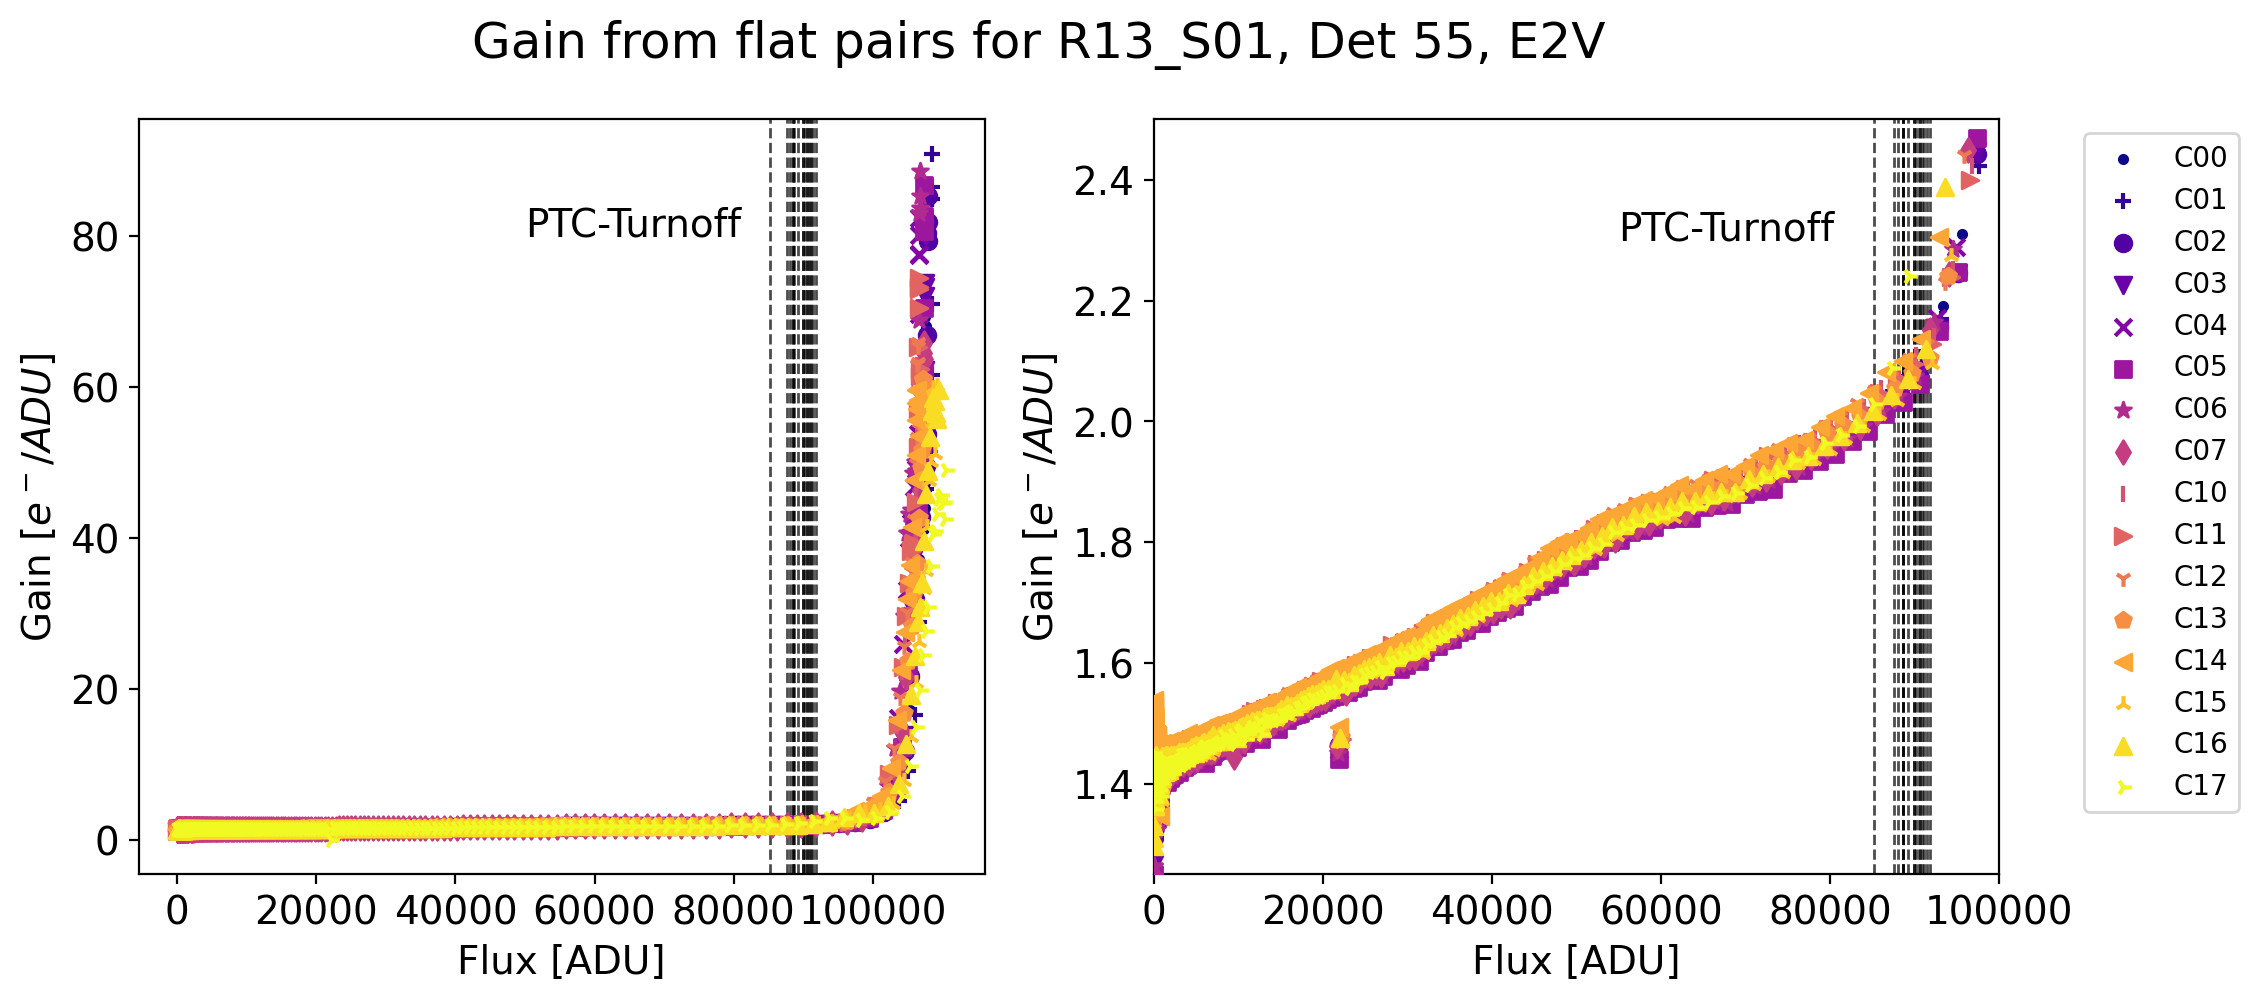
\includegraphics[width=\textwidth]{Figures/Gain_plot_55.png}
    \caption{Gain values obtained by flat pairs for fluxes up to approximately 120000 ADU for detector 55 (R13\_S01). In both panels, the dashed vertical lines represent the PTC turnoff value for each of the 16 detector segments, and the colored figures represent the gain and flux values for each segment. The right panel shows only the region up to the PTC-turnoff of the left panel.}
    \label{fig:Gain_full}
\end{figure}

\vspace{3mm}

As we mentioned in the methodology (sec. \ref{sec:methods}), we used two code versions (w\_2022\_27 and w\_2022\_32), where the main difference and our interests is the one shown in figure \ref{fig:diff_codes}. This figure shows how the two code versions handled the statistics to compute gain by pairs of flats. The \textit{w\_202222\_27} version used the red code with the assumption of a Gaussian distribution, so it truncates the distribution to reject outliers. Whereas the \textit{w\_2022\_32} version used the green code rejecting the before assumption. The last one is our recommendation due to the analysis results described in this section. In short: the distribution of the operation between two flats images leading to calculating the gain does not have a Gaussian distribution, so performing a truncation in the distribution alters the expected value for the gain.


\begin{figure}[!htb]
    \centering
    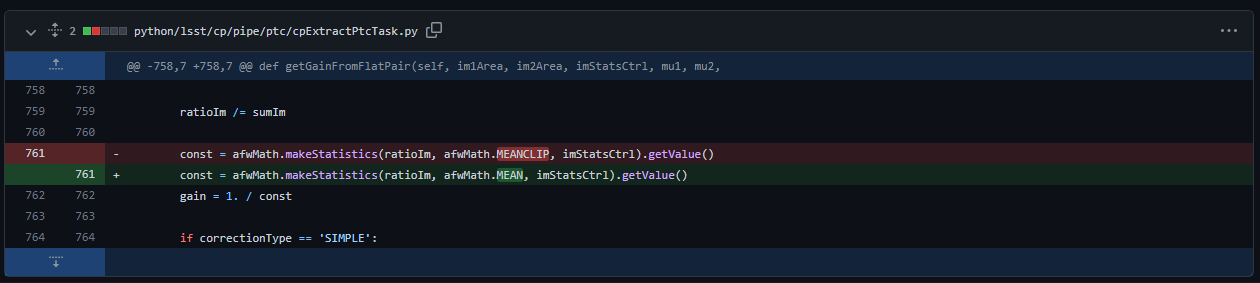
\includegraphics[width=\textwidth]{Figures/Cambio_codigo.png}
    \caption{Difference between the initial(w\_2022\_27, in red) and current (w\_2022\_32, in green) codes for calculating the gain from a pair of flat fields.}
    \label{fig:diff_codes}
\end{figure}

The version \textit{w2022} gave us the result shown in figure \ref{fig:relative_error_oldcode}, a relative percentage error between the gain per PTC and flat pair at a flux of 5000 ADU above 5 \%, the same result for an E2V detector (upper panel) and an ITL detector (lower panel). This high percentage at this flux was not expected, so we performed simulations with the methodology described in section \ref{subsubsec:method_Simulation_Gain} to investigate what was generating this value.


\subsubsection{Simulation}

From the previous result, a relative error between the gains of 5 \% at 5000 ADU, we had some hypotheses: first, the masks in the flat images could be affecting in some way, e.g.,  if the masks of each image are very different and the code uses these to make calculations, it could generate a high relative error; second, an overestimation in the read noise; and third, if it is not the masks, so what in the statistics is causing this error. 

\vspace{3mm}

We found from simulations of a flat image of a CCD segment and using the mask of an actual segment: the use of one mask for the two flats, the union of both masks, or different masks for each do not account for the error of 5 \% at 5000 ADU, as shown in the top panel of Figure \ref{fig:simulation_masks}. We notice in this case that the higher the read noise, when using a NONE type correction, the more significant the discrepancies between the expected and calculated gain (2 $e^-$/ADU). However,  the subsequent corrections (SIMPLE and FULL), which account for the read noise, accurately calculate the expected gain value. Nonetheless,  the bottom panel of this figure, which includes, besides the masks, the control statistics, gives an account in all cases of a relative percentage error between the gain per PTC and flats pairs above 5 \%. In the next section (\ref{subsubsec:results_gainflats_realdata}) we check this with the real data.

%Encontramos a partir de las simulaciones de la imagen flat de un segmento de CCD, utilizando una máscara de un segmento real, que utilizar una máscara para los dos flats, la unión de ambas máscaras o máscaras diferentes para cada uno, no daba cuenta del error del 5\% a 5000 ADU, tal y como lo muestra el panel superior de la figura \ref{fig:simulation_masks},lo único que podemos ver en este caso es que a mayor ruido de lectura, y al utilizar una corrección de tipo NONE, mayores son las discrepancias entre la ganancia esperada (2 $e^-$/ADU) y la calculada, pero las subsecuentes correcciones (SIMPLE y FULL) que sí tienen en cuenta el valor del ruido de lectura logran calcular de forma precisa el valor esperado de ganancia. No obstante, el panel inferior de esta figura, que incluye además de las máscaras estadísticos de control, me da cuenta en todos los casos de un error relativo porcentual entre la ganancia por PTC y pares de flats por encima del 5 \%. En la siguiente sección (\ref{subsubsec:results_gainflats_realdata}) comprobamos esto con los datos reales.



\begin{figure}[!htb]
     \centering
     \begin{subfigure}[b]{\textwidth}
         \centering
         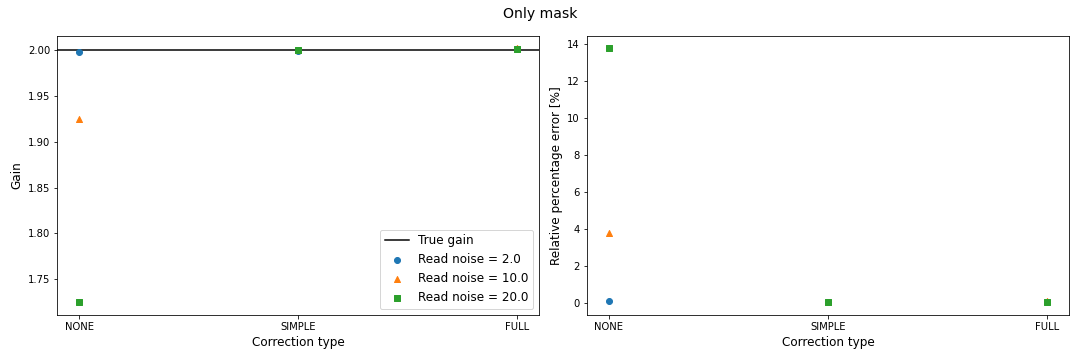
\includegraphics[width=\textwidth]{Figures/Simulation_masks.png}
     \end{subfigure}
     \vspace{3mm}
     \begin{subfigure}[b]{\textwidth}
         \centering
         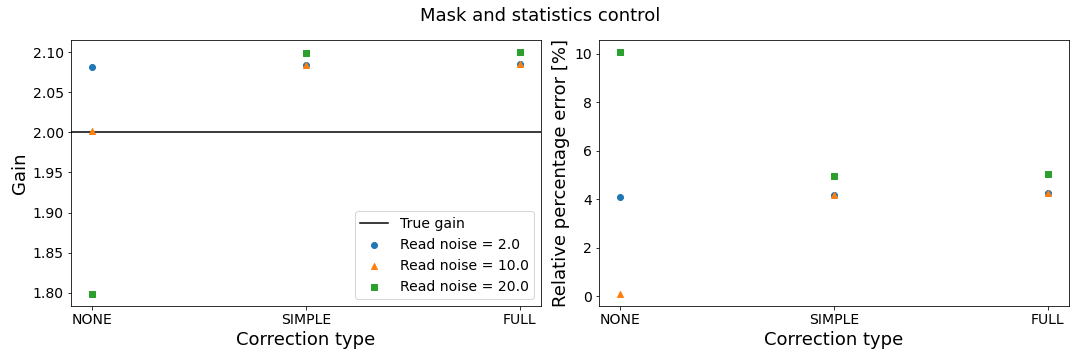
\includegraphics[width=\textwidth]{Figures/Simulation_masks_stats.png}
     \end{subfigure}
        \caption{Simulation results to obtain the gain per pair of flats in the upper panel using only masks and in the lower panel adding control statistics. The average flux value of these simulated flats is $5000$. The left panels show the gain value for three different models, and on the right, the relative percent error concerning the expected gain value, 2 $e^-/$ADU. In the left panels, the horizontal black line represents the predicted gain value, and the figures represent the different values considered for the read noise: the blue circle of 2 $e^-$, the orange triangle of 10 $e^-$, and the green square of 20$e^-$. Considering these read noises, we calculated the gain for three models: NONE, SIMPLE and FULL.}
        %Resultados de la simulación para obtener la ganancia por pares de flats, en el panel superior utilizando únicamente máscaras y en el inferior añadiendo además estadísticos de control. El valor promedio de flujo de estos flats simulados es de $\sim 5000$. Los paneles de la izquierda muestran el valor de la ganancia para 3 diferentes modelos y a la derecha el error relativo porcentual respecto al valor esperado de ganancia, 2 $e^-/$ADU. En los paneles izquierdos la línea negra horizontal representa el valor de ganancia esperado y las figuras representan los diferentes valores considerados para el ruido de lectura: círculo azul de 2 $e^-/$, triángulo naranja de 10 $e^-/$ y cuadrado verde de 20$e^-/$. Considerando estos ruidos de lectura se calculó la ganancia para tres modelos diferentes: NONE, SIMPLE y FULL.}
        \label{fig:simulation_masks}
\end{figure}

\subsubsection{Real data} \label{subsubsec:results_gainflats_realdata}
 
 Because of the results obtained from the simulation, we checked whether the results held with the actual data, and indeed they did. We performed this check on detector 55 (R13\_S01) for all its segments, as shown in figures \ref{fig:GainFlats_NOstats} and \ref{fig:GainFlats_stats}, where the black crosses represent the gain value obtained from the PTC. The first figure again reveals that the masks and no control statistics do not account for a relative error more significant than 5 \% for any segment of the detector; indeed, the maximum value achieved is 2.25 \% at an average flux of 5450 ADU. In the before result, we used the same mask for calculations: the union of the individual masks. The second figure, which uses the masks and incorporates the control statistics, shows that the handling of the statistics is producing high discrepancies between the gain by PTC and pairs of flats, reaching differences of up to 9 \% in one of the segments at a flow rate of 5450 ADU.
 
%En vista de los resultados obtenidos a partir de la simulación, se verificó si los resultados se mantienen con los datos reales y en efecto lo hacen. Hicimos esta comprobación en el detector 55 (R13\_S01) para todos sus segmentos, como se muestra en las figuras \ref{fig:GainFlats_NOstats} y \ref{fig:GainFlats_stats}, donde las cruces negras representan el valor de ganancia obtenida a partir de la PTC. La primera figura nuevamente revela que el uso de las máscaras (misma máscara utilizada para los cálculos, que es la unión de las máscaras individuales) y sin estadísticos de control no da cuenta de un error relativo mayor al 5 \% para ningún segmento del detector, el máximo valor alcanzado es de 2.25 \% a un flujo promedio de 5450 ADU. La segunda figura, que incorpora además los estadísticos de control, en cambio muestra que, en efecto, el manejo de los estadísticos está produciendo altas discrepancias entre la ganancia por PTC y la ganancia calculada por pares de flats llegando a alcanzar diferencias hasta del 9 \% en uno de los segmentos a un flujo de 5450 ADU.
 
\begin{figure}[!htb]
    \centering
    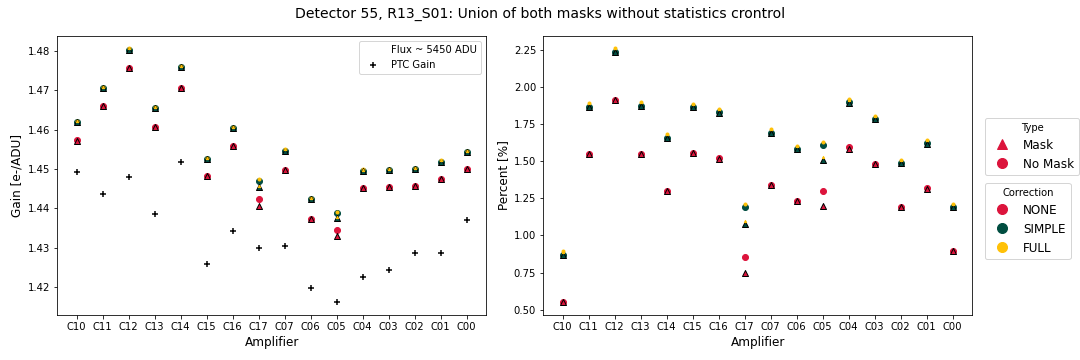
\includegraphics[width=\textwidth]{Figures/GainFlats_NOstats_det55.png}
    \caption{Gain value on the left panel and the relative percentage error on the right panel for the 16 segments (amplifiers) of detector 55 (R13\_S01). In the left panel, the black crosses represent the value of the gain per PTC. For both panels, the figures represent whether the calculation of the gain from flat pairs used mask (triangles) or not (circles) and the colors are associated with the model used to determine the gain: NONE (red), SIMPLE (green) and FULL (yellow). The mask for calculation was the union of the masks of both flat images per segment, and we did not use control statistics.}
    %Valor de ganancia (panel izquierdo) y error relativo porcentual (panel derecho) para los 16 segmentos (amplifier) del detector 55 (R13\_S01). En el panel izquierdo las cruces negras representan el valor de la ganancia por PTC. Para ambos paneles las figuras representan si el cálculo de la ganancia por pares de flats utilizó máscara (triángulos) o si no la utilizó (círculos), y los colores están asociados al modelo empleado para determinar la ganancia: NONE, SIMPLE y FULL. Para la máscara se utilizó la unión de las máscaras de ambas imágenes flat por segmento y no se utilizó estadísticos de control.}
    \label{fig:GainFlats_NOstats}
\end{figure}

\begin{figure}[H]
    \centering
    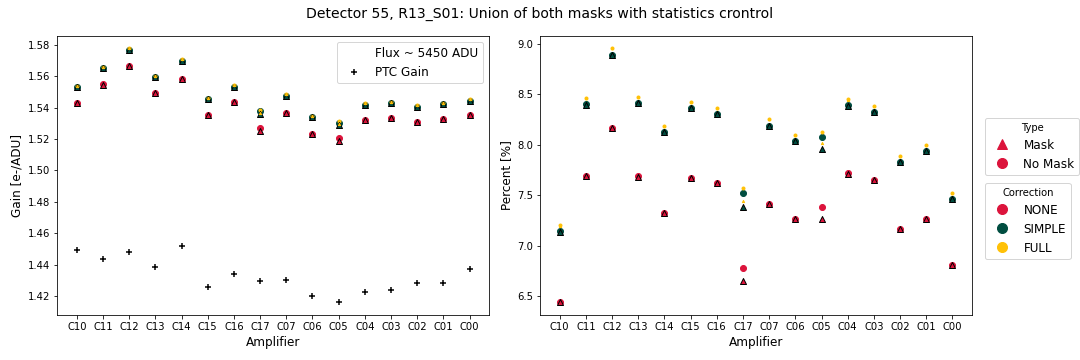
\includegraphics[width=\textwidth]{Figures/GainFlats_stats_det55.png}
    \caption{See description of the figure \ref{fig:GainFlats_NOstats}. This figure used control statistics.}
    \label{fig:GainFlats_stats}
\end{figure}
 
 
Subsequently, we performed plots of the distributions for the operation between the flats images given by the equation \ref{eq:ratioIm}, which is the argument of the Lupton equation (eq. \ref{eq:Lupton}) and is directly related to the gain. The results we obtained are shown in figure \ref{fig:hist_ratioIM} for each detector segment and reveal that the shape of this distribution is far from Gaussian. So truncating this distribution produces a change in the mean value, which no longer coincides with the mean of the original distribution, thus giving a different gain value than expected. 

\vspace{3mm}

Finally, we again constructed the relative percentage error figures for the gain without truncating the distribution, as shown by the green code in figure \ref{fig:diff_codes}. We obtained the result in figure \ref{fig:relative_error}, which reveals in its embedded image that for a flow of 5000 ADU, the difference between the two gains is now below 5 \%, as indicated by the simulations. With this result, we estimate a general relationship for the gain taking into account the distributions for the linear fit parameters, as shown in figure \ref{fig:histogram_linearfit}, which was performed between 5000 and 10000 ADU. In this figure, we can see on the top left the distribution of the slopes by the vendor, which reveals a clear bimodality, with the E2V detectors having a slightly higher slope concerning ITL, with a mean of $(0.00046 \pm 0.00004)$ and $(0.00027 \pm 0.00004)$ \%/ADU, respectively. In the bottom panel of this figure, we have the intercept with the y-axis (i.e., with the percentage error axis between the gains), and it shows that there is an overall mean across the detectors, with no appreciable distinction by vendor, with a value of $(-0.5 \pm 0.5)$ \%. Thus, by vendor, the relative percentage error between the 5000 and 1000 ADU is given by


%Finalmente, sin efectuar truncamiento en la distribución, como lo muestra el código en verde de la figura \ref{fig:diff_codes}, construimos nuevamente las figuras de error relativo porcentual para la ganancia y obtuvimos el resultado de la figura \ref{fig:relative_error} que revela en su imagen embebida que para un flujo de 5000 ADU que la diferencia entre ambas ganancias ahora está por debajo del 5 \% como lo indicaban las simulaciones. Con este resultado estimamos una relación general para la ganancia teniendo en cuntra las distribuciones para los parámetros del ajuste lineal, como se muestran en la figura \ref{fig:histogram_linearfit}, que fue efectuado entre los 5000 y 10000 ADU. En esta figura se observa a la izquierda arriba la distribución de las pendiente por fabricante que revela una clara bimodalidad, teniendo una pendiente ligeramente mayor los detectores de E2V respecto a ITL, con una media de $(0.00046 \pm 0.00004)$ y $(0.00027 \pm 0.00004)$ \%/ADU, respectivamente. En el panel inferior de esta figura tenemos el intercepto con el eje y (es decir, con el eje del porcentaje de error entre las ganancias) y muestra que hay una media global en los detectores, sin distinción apreciable por fabricante, con un valor de $(-0.5 \pm 0.5)$ \%. Así las cosas, por fabricante, el error relativo porcentual entre los 5000 y 1000 ADU está dado por

\begin{itemize}
    \item E2V: $Error_{2Gain} = (0.00046 \pm 0.00004) F - (0.5 \pm 0.5)$, where the error interval is ($1.8 \pm 0.7$, $4.1 \pm 0.9$) \%.
    \item ITL: $Error_{2Gain} = (0.00027 \pm 0.00004) F - (0.5 \pm 0.5)$, where the error interval is ($0.85 \pm 0.7$, $2.2 \pm 0.9$) \%.
\end{itemize}
 
\begin{figure}[!htb]
    \centering
    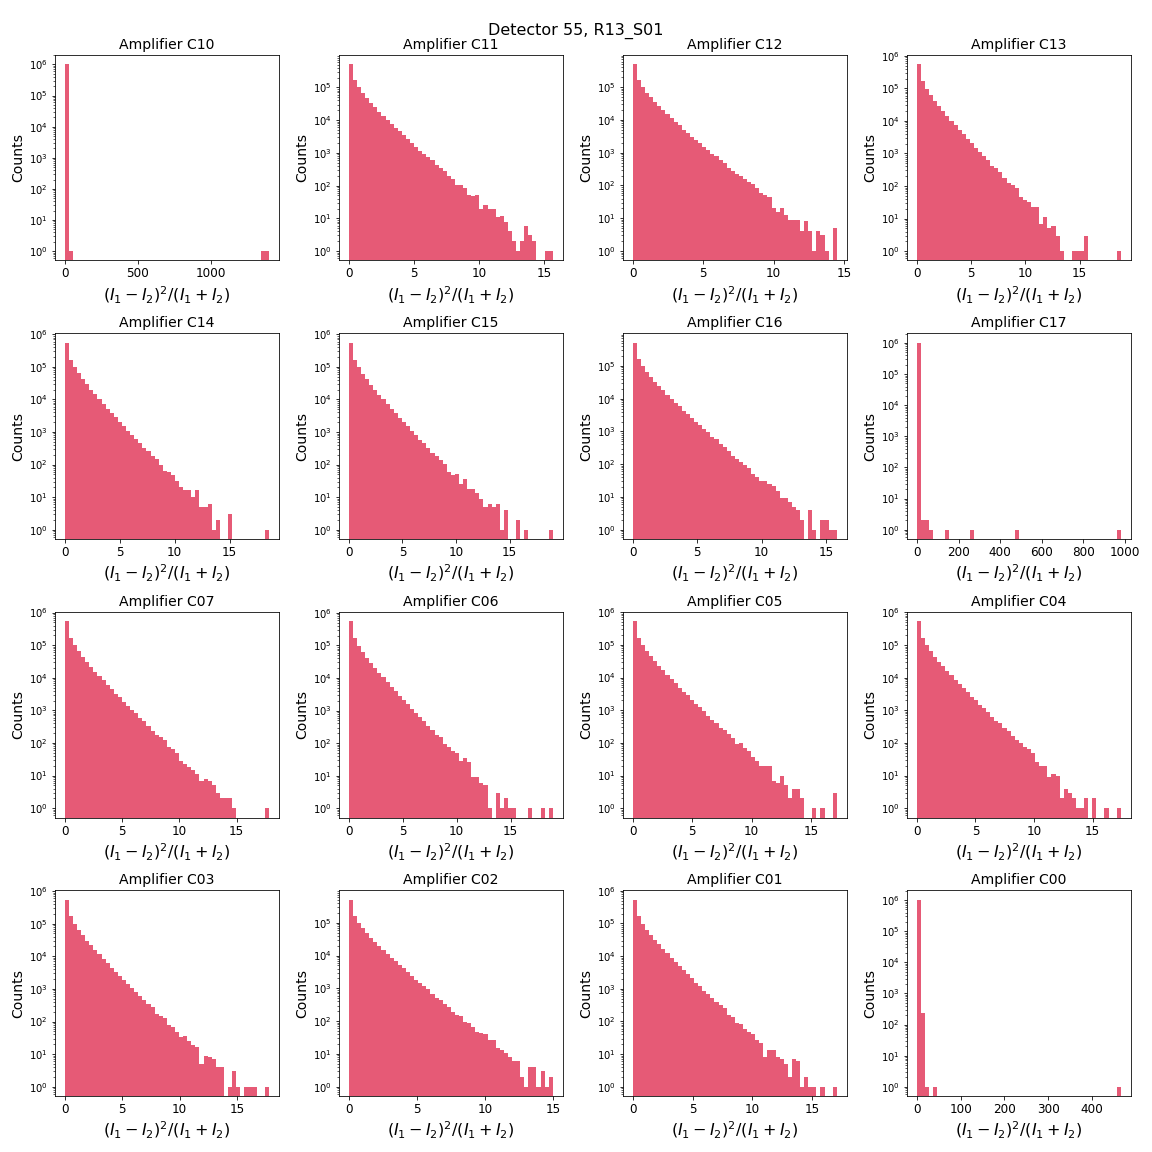
\includegraphics[width=\textwidth]{Figures/Histogram_ratioIM_det55.png}
    \caption{Histogram of the distribution for $\frac{(I_1 - I_2)^2}{I_1 + I_2}$ for each segment of detector 55 (R13\_S01). }
    \label{fig:hist_ratioIM}
\end{figure}


\begin{figure}[!htb]
     \centering
     \begin{subfigure}[b]{\textwidth}
         \centering
         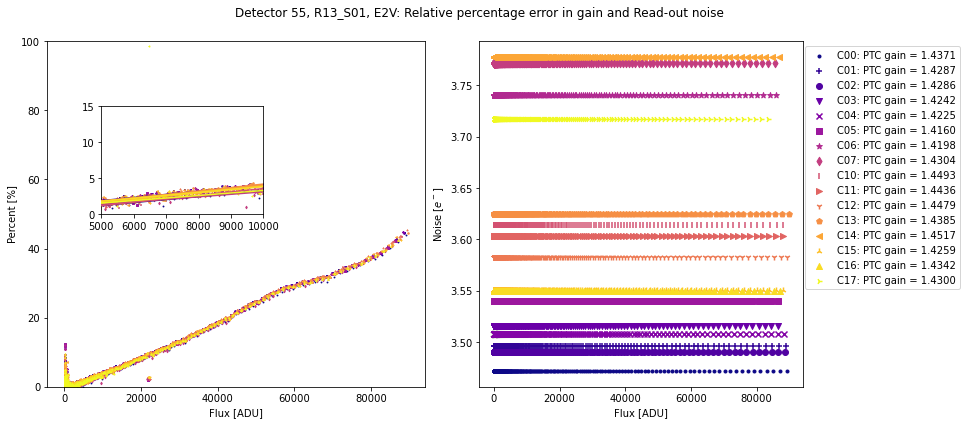
\includegraphics[width=\textwidth]{Figures/Relative_Error_Gain_Noise_detectorR13_S01.png}
     \end{subfigure}
     \vspace{3mm}
     \begin{subfigure}[b]{\textwidth}
         \centering
         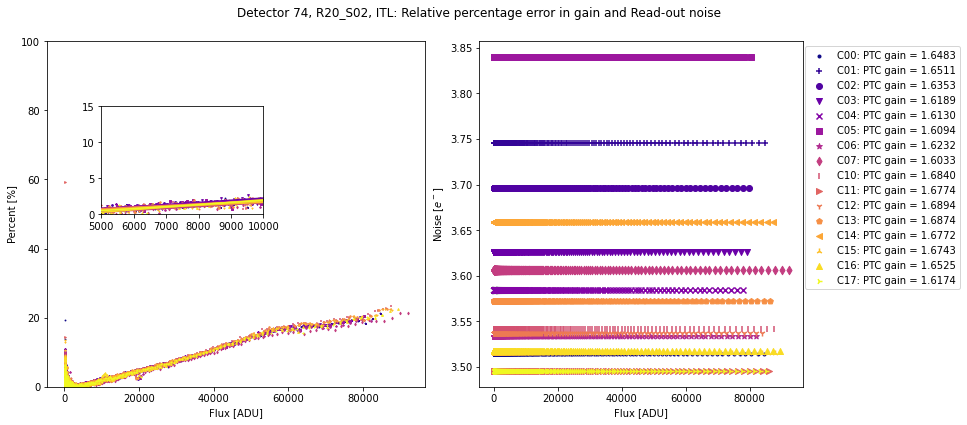
\includegraphics[width=\textwidth]{Figures/Relative_Error_Gain_Noise_detectorR20_S02.png}
     \end{subfigure}
        \caption{Refer to the description of the figure \ref{fig:relative_error_oldcode}. This plot uses the updated code (version w\_2022\_32) that does not use clipped mean.}
        \label{fig:relative_error}
\end{figure}

\begin{figure}[!htb]
     \centering
     \begin{subfigure}[b]{\textwidth}
         \centering
         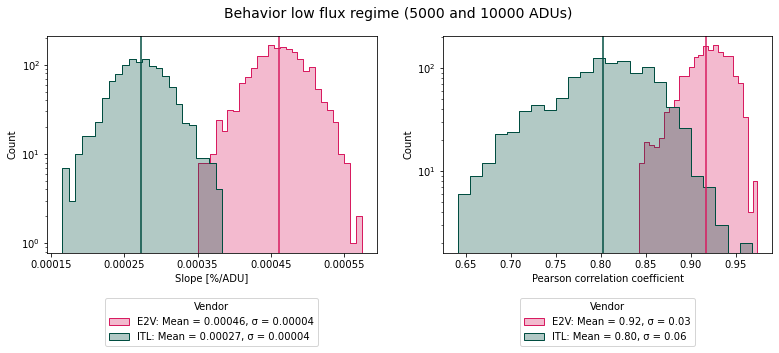
\includegraphics[width=\textwidth]{Figures/Histogram_slope_corr_new.png}
     \end{subfigure}
     \vspace{3mm}
     \begin{subfigure}[b]{\textwidth}
         \centering
         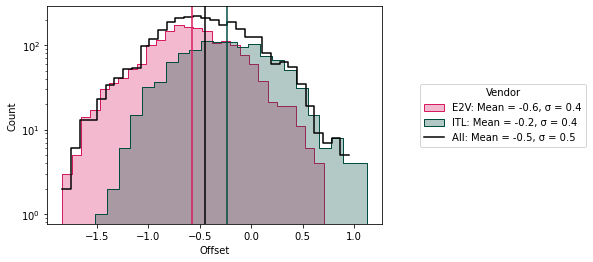
\includegraphics[width=0.7\textwidth]{Figures/Histogram_offset_new.png}
     \end{subfigure}
        \caption{Histograms for the slope (top left), Pearson's correlation coefficient (top right), and the y-axis intercept (offset, bottom panel) corresponding to the linear fit performed in the flow region between 5000 and 10000 ADU for the gain. Its construction used the updated code (version w\_2022\_32), and the colors represent the vendor, E2V in red and ITL in blue. The vertical lines represent the mean for each case.  }
        \label{fig:histogram_linearfit}
\end{figure}

\subsection{Crosstalk and non linearity correction} \label{subsec:crosstalk_and_linearity}

A part of the final analyses we performed during this internship consisted of quantifying and deciding whether the crosstalk effect and the nonlinearity impact the shape of the PTC and/or the fundamental parameters: gain, read noise, B-F effect, and turnoff coefficient.
%Parte de los análisis finales que efectuamos durante esta pasantía consistió en cuantificar y decidir si el efecto de crosstalk y la no linealidad tienen impacto en la forma de la PTC y/o de los parámetros fundamentales: ganancia, ruido de lectura, coeficiente del B-F effect y turnoff. 

\vspace{3mm}

As described in section \ref{subsec:method_Crosstalk}, we had access to the crosstalk matrices for detector 32 (ITL) and 139 (E2V), which are shown in Figure \ref{fig:crosstalk_matrix}. We obtained from applying the methodology of that section that the differences between PTC with and without crosstalk correction are shallow, as shown in Figure \ref{fig:crosstalk_corr32} and Figure \ref{fig:crosstalk_corr139}. They illustrated that considering the region below saturation, the difference between the variances is consistently below 0.1 ADU. In contrast, the most significant variance in the parameters is $\sim 0.1$\% in read noise and BF effect coefficient and  $\sim 0.07$ \% in gain and turnoff. The most significant differences were found in the ITL detector segments. According to the above, we conclude that the crosstalk does not have a considerable effect. So, correcting this effect is unnecessary since the difference in the parameters is small and does not alter the shape of the PTC.  

%Como se describió en la sección \ref{subsec:method_Crosstalk}, tuvimos acceso a las matrices de crosstalk para el detector 32 (ITL) y el 139 (E2V), que se muestran en las figura \ref{fig:crosstalk_matrix}. Como resultado de la metodología de dicha sección obtuvimos que las diferencias de la PTC corregida y no corregida por crosstalk es muy baja, como se muestra en las figura \ref{fig:crosstalk_corr32} y \ref{fig:crosstalk_corr139}, donde se muestra que considerando la región por debajo de saturación, la diferencia entre las varianzas está por debajo siempre de 0.1 ADU, mientras que en los parámetros la mayor variación es de $\sim 0.1$\% en el ruido de lectura y en el coeficiente del B-F effect y $\sim 0.07$ \% en la ganancia y el turnoff. Las mayores diferencias se encontraron en los segmentos del detector de ITL. De acuerdo con lo anterior, llegamos a la conclusión de que el crosstalk no tiene un efecto importante y no es necesario corregir por este efecto ya que la diferencia en los parámetros es pequeña y no altera la forma de la PTC.  



\begin{figure}[!htb]
    \centering
    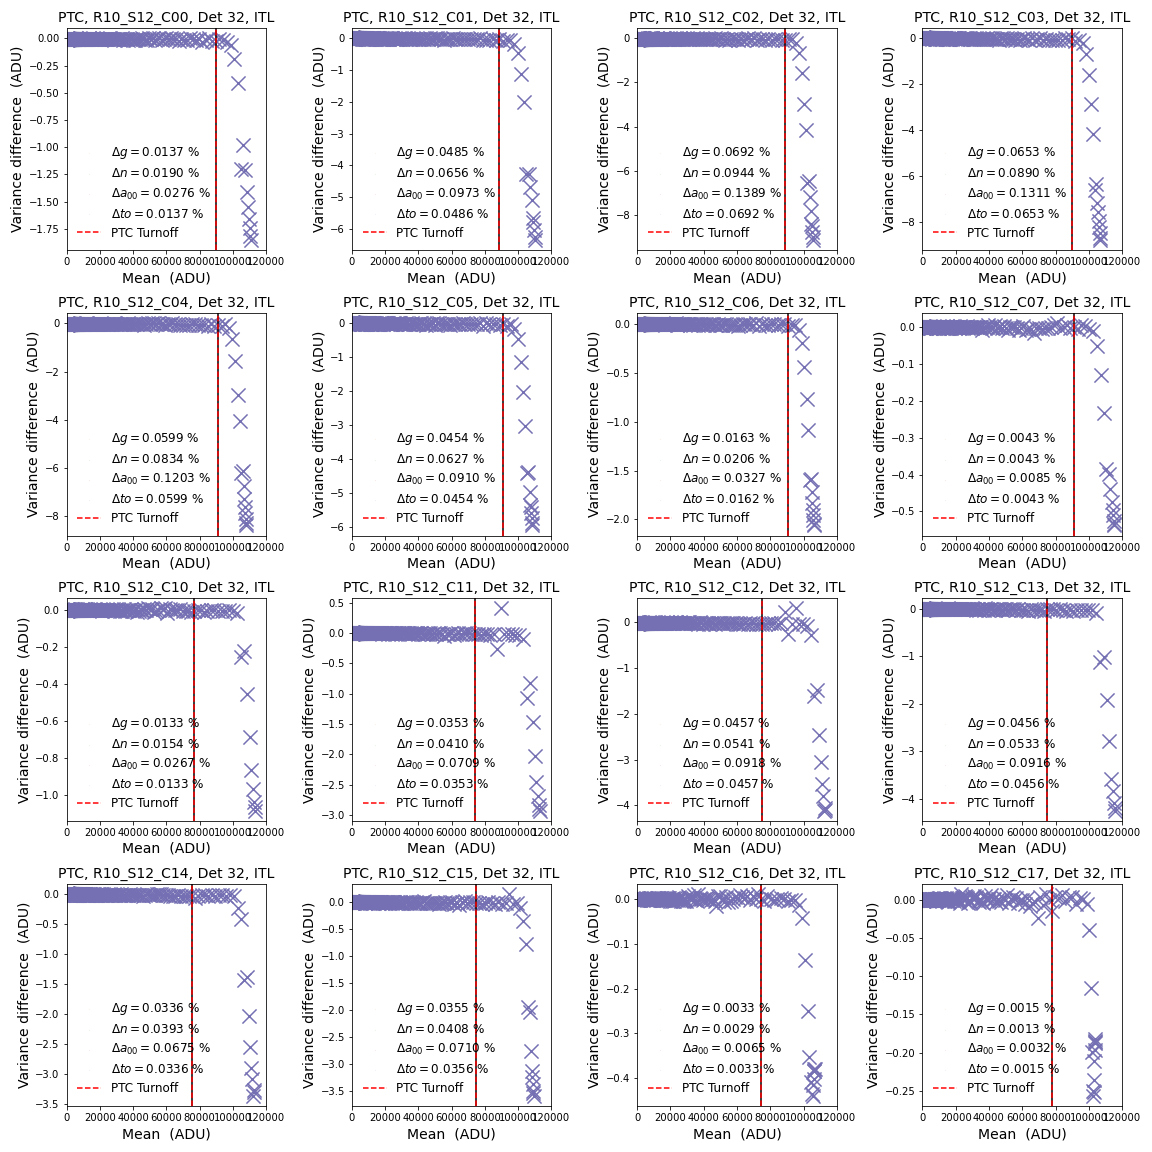
\includegraphics[width=\textwidth]{Figures/ptc_crosstalk32.png}
    \caption{The plot of the variance difference vs. mean for detector 32 (R10\_S12) for vendor ITL, where the variance difference is between the variance value without and with crosstalk correction. This is shown for each CCD segment, where the vertical lines mark the  PTC-turnoff values. In the legends, we displayed the differences between the parameters:  $\Delta g$ for the gain, $\Delta n$ for the read noise, $\Delta a_{00}$ for the brighter-fatter effect coefficient, and $\Delta to$ for the PTC-turnoff.}
    %Gráfica de la diferencia de varianza vs la media para el detector 32 (R10\_S12) para el fabricante ITL, donde la diferencia de varianza es entre el valor de varianza sin y con corrección por crosstalk. Se muestra esto para cada uno de los segmentos del CCD, mostrando por la línea vertical los valores de PTC-turnoff y en las respectivas leyendas las diferencias entre los parámetros: $\Delta g$ para la ganancia, $\Delta n$ para el ruido de lectura, $\Delta a_{00}$ para el coeficiente del brigther-fatter effect y $\Delta to$ para el PTC-turnoff.}
    \label{fig:crosstalk_corr32}
\end{figure}

\begin{figure}[!htb]
    \centering
    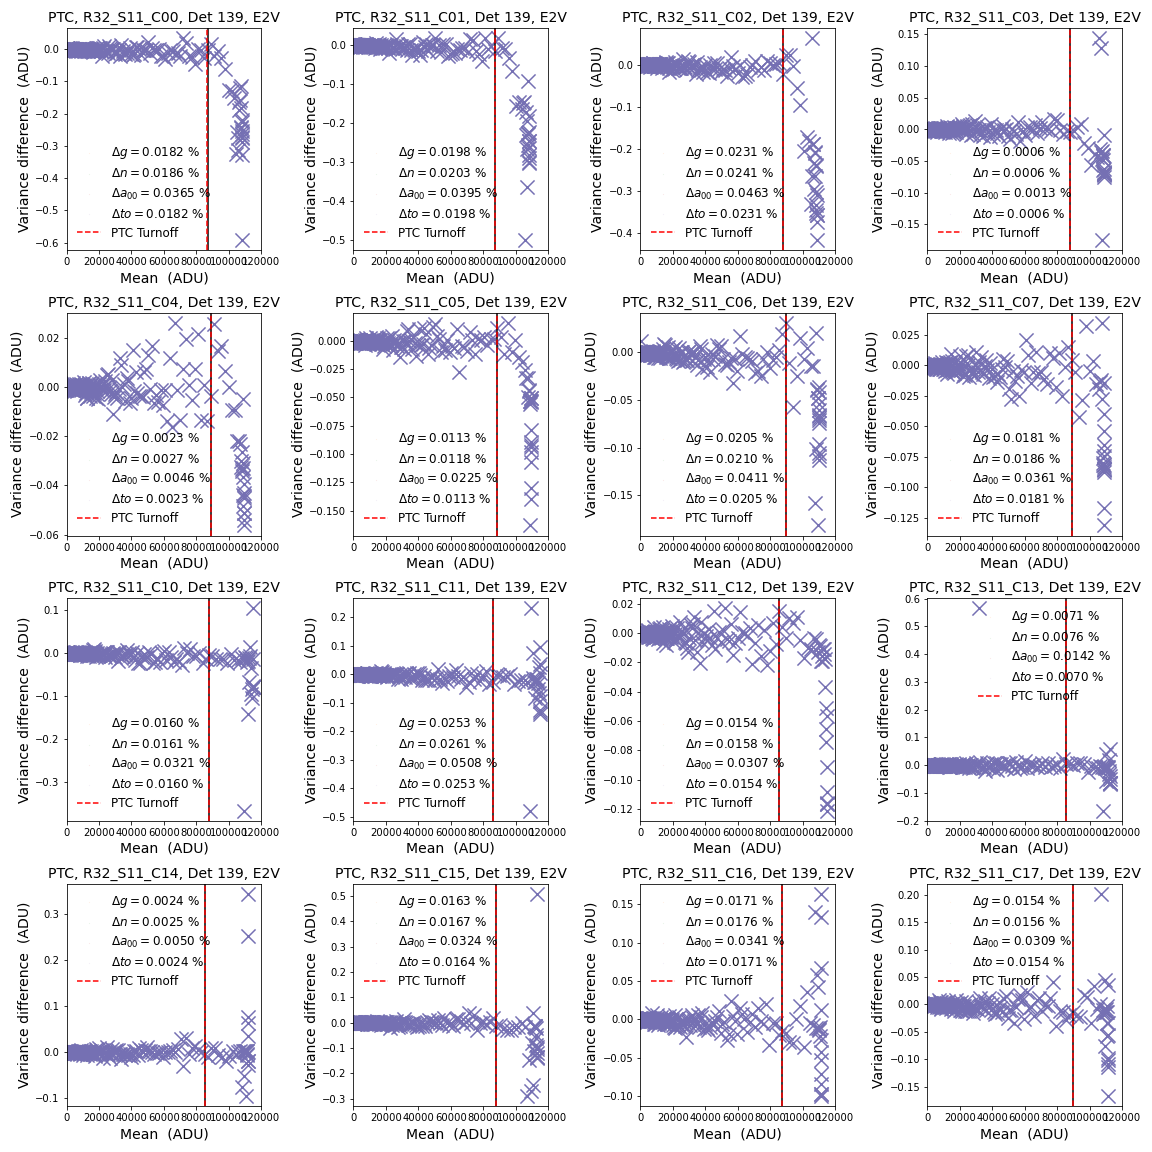
\includegraphics[width=\textwidth]{Figures/ptc_crosstalk139.png}
    \caption{Refer to the description of the figure \ref{fig:crosstalk_corr32}. This plot is for detector 139 (R32\_S11) for vendor E2V.}
    \label{fig:crosstalk_corr139}
\end{figure}

Finally, the 12-node cubic spline linearizer was applied to verify its impact on the PTC shape. The result of correcting only for crosstalk (orange dots), only for nonlinearity (blue diamonds), corrected for both effects (gray triangles), and the uncorrected data (magenta squares) is presented in Figure \ref{fig:varmean_crosstalk}. We see that the uncorrected data show a bump around 60000 ADU, while the crosstalk-corrected data are always located at the same position as the uncorrected data (thus also showing the bump),the data corrected for nonlinearity flatten it. Accordingly, making both corrections to the data has no more significant effect than fixing for nonlinearity alone. Again we find that the crosstalk is not a necessary correction since it does not affect either the shape or the parameters of the PTC. 

%Finalmente, se aplicó el linealizador spline cúbico de 12 nodos para verificar su impacto en la forma de la PTC. Se presenta en la figura \ref{fig:varmean_crosstalk} el resultado de corregir solo por crosstalk (puntos naranja), solo por la no linealidad (diamantes azules), corregidos por ambos efectos (triángulos grises) y los datos sin corregir (cuadrados magenta). Vemos que los datos sin corregir presentan un bache alrededor de los 60000 ADU, mientras que los datos corregidos por crosstalk se ubican siempre en la misma posición de los datos no corregidos (por tanto también muestran el bache), los datos corregidos por la no linealidad lo aplanan. De acuerdo con lo anterior, hacer las dos correcciones a los datos no tiene mayor efecto al que se obtiene corrigiendo solamente por la no linealidad. Nuevamente comprobamos que el crosstalk no es una corrección necesaria dado que no afecta ni la forma, ni los parámetros de la PTC. 


\begin{figure}[!htb]
     \centering
     \begin{subfigure}[b]{0.49\textwidth}
         \centering
         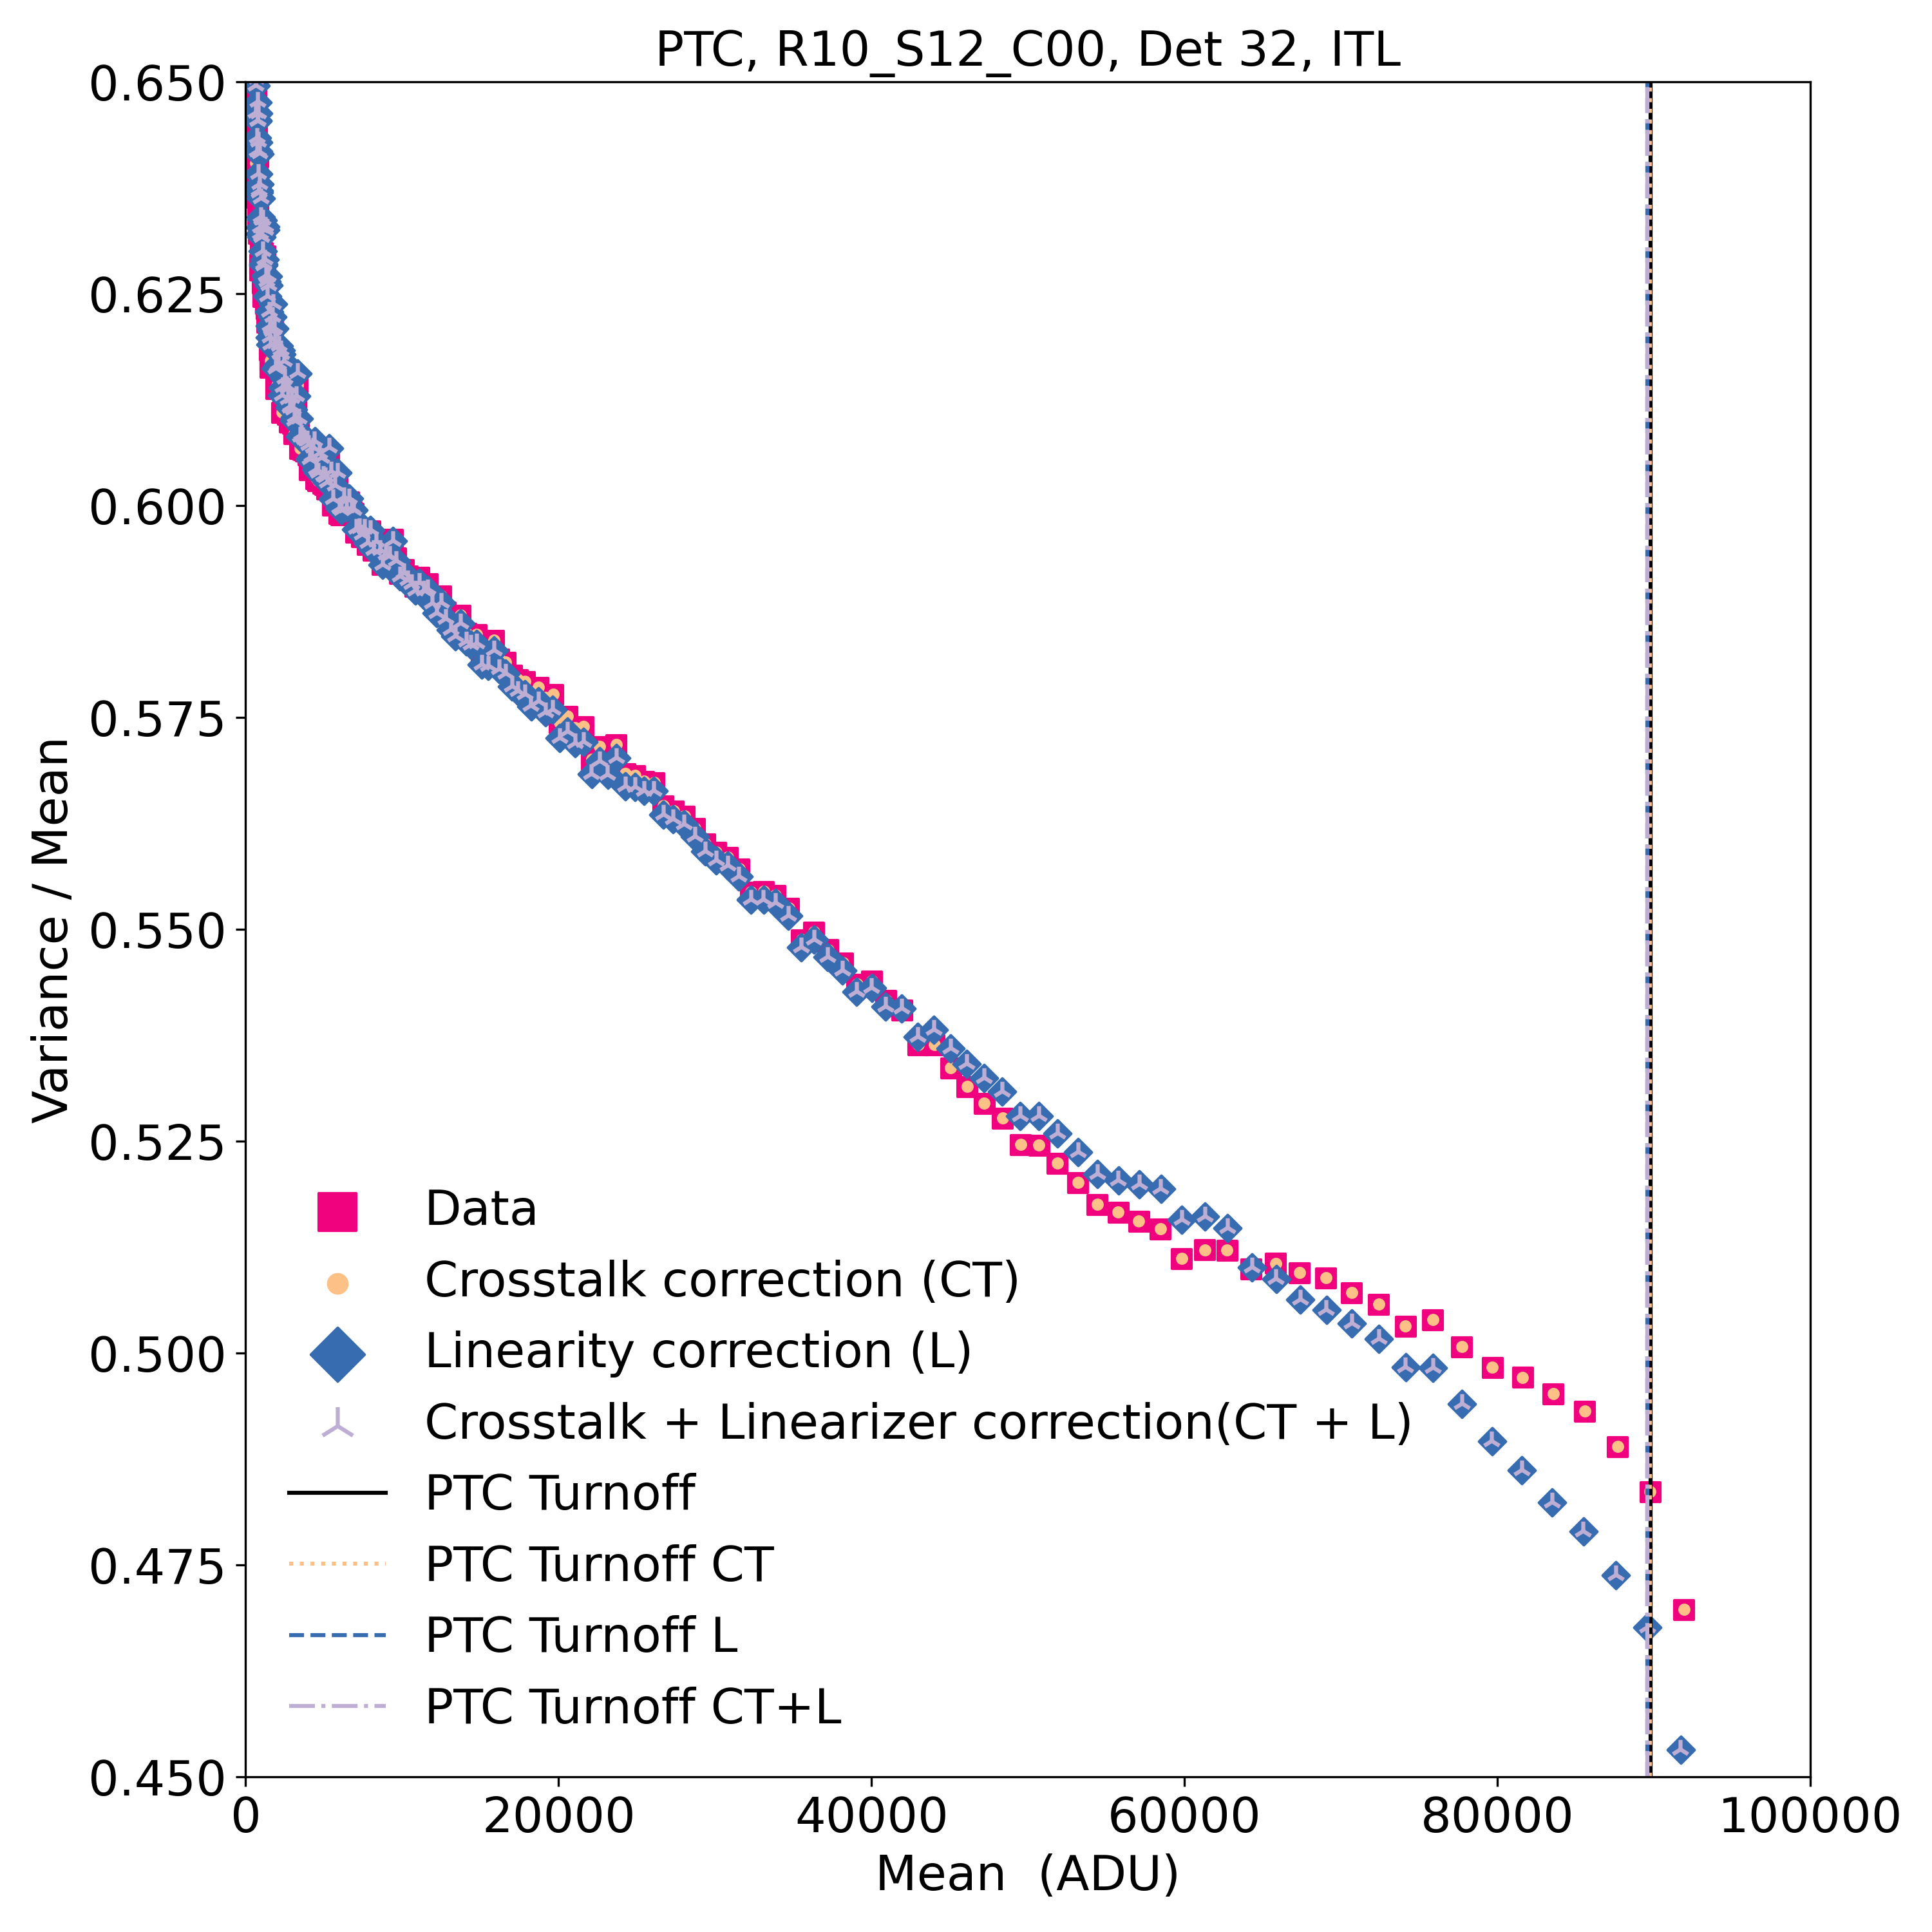
\includegraphics[width=\textwidth]{Figures/Variance_Mean_vs_Mean32.png}
     \end{subfigure}
     \hfill
     \begin{subfigure}[b]{0.49\textwidth}
         \centering
         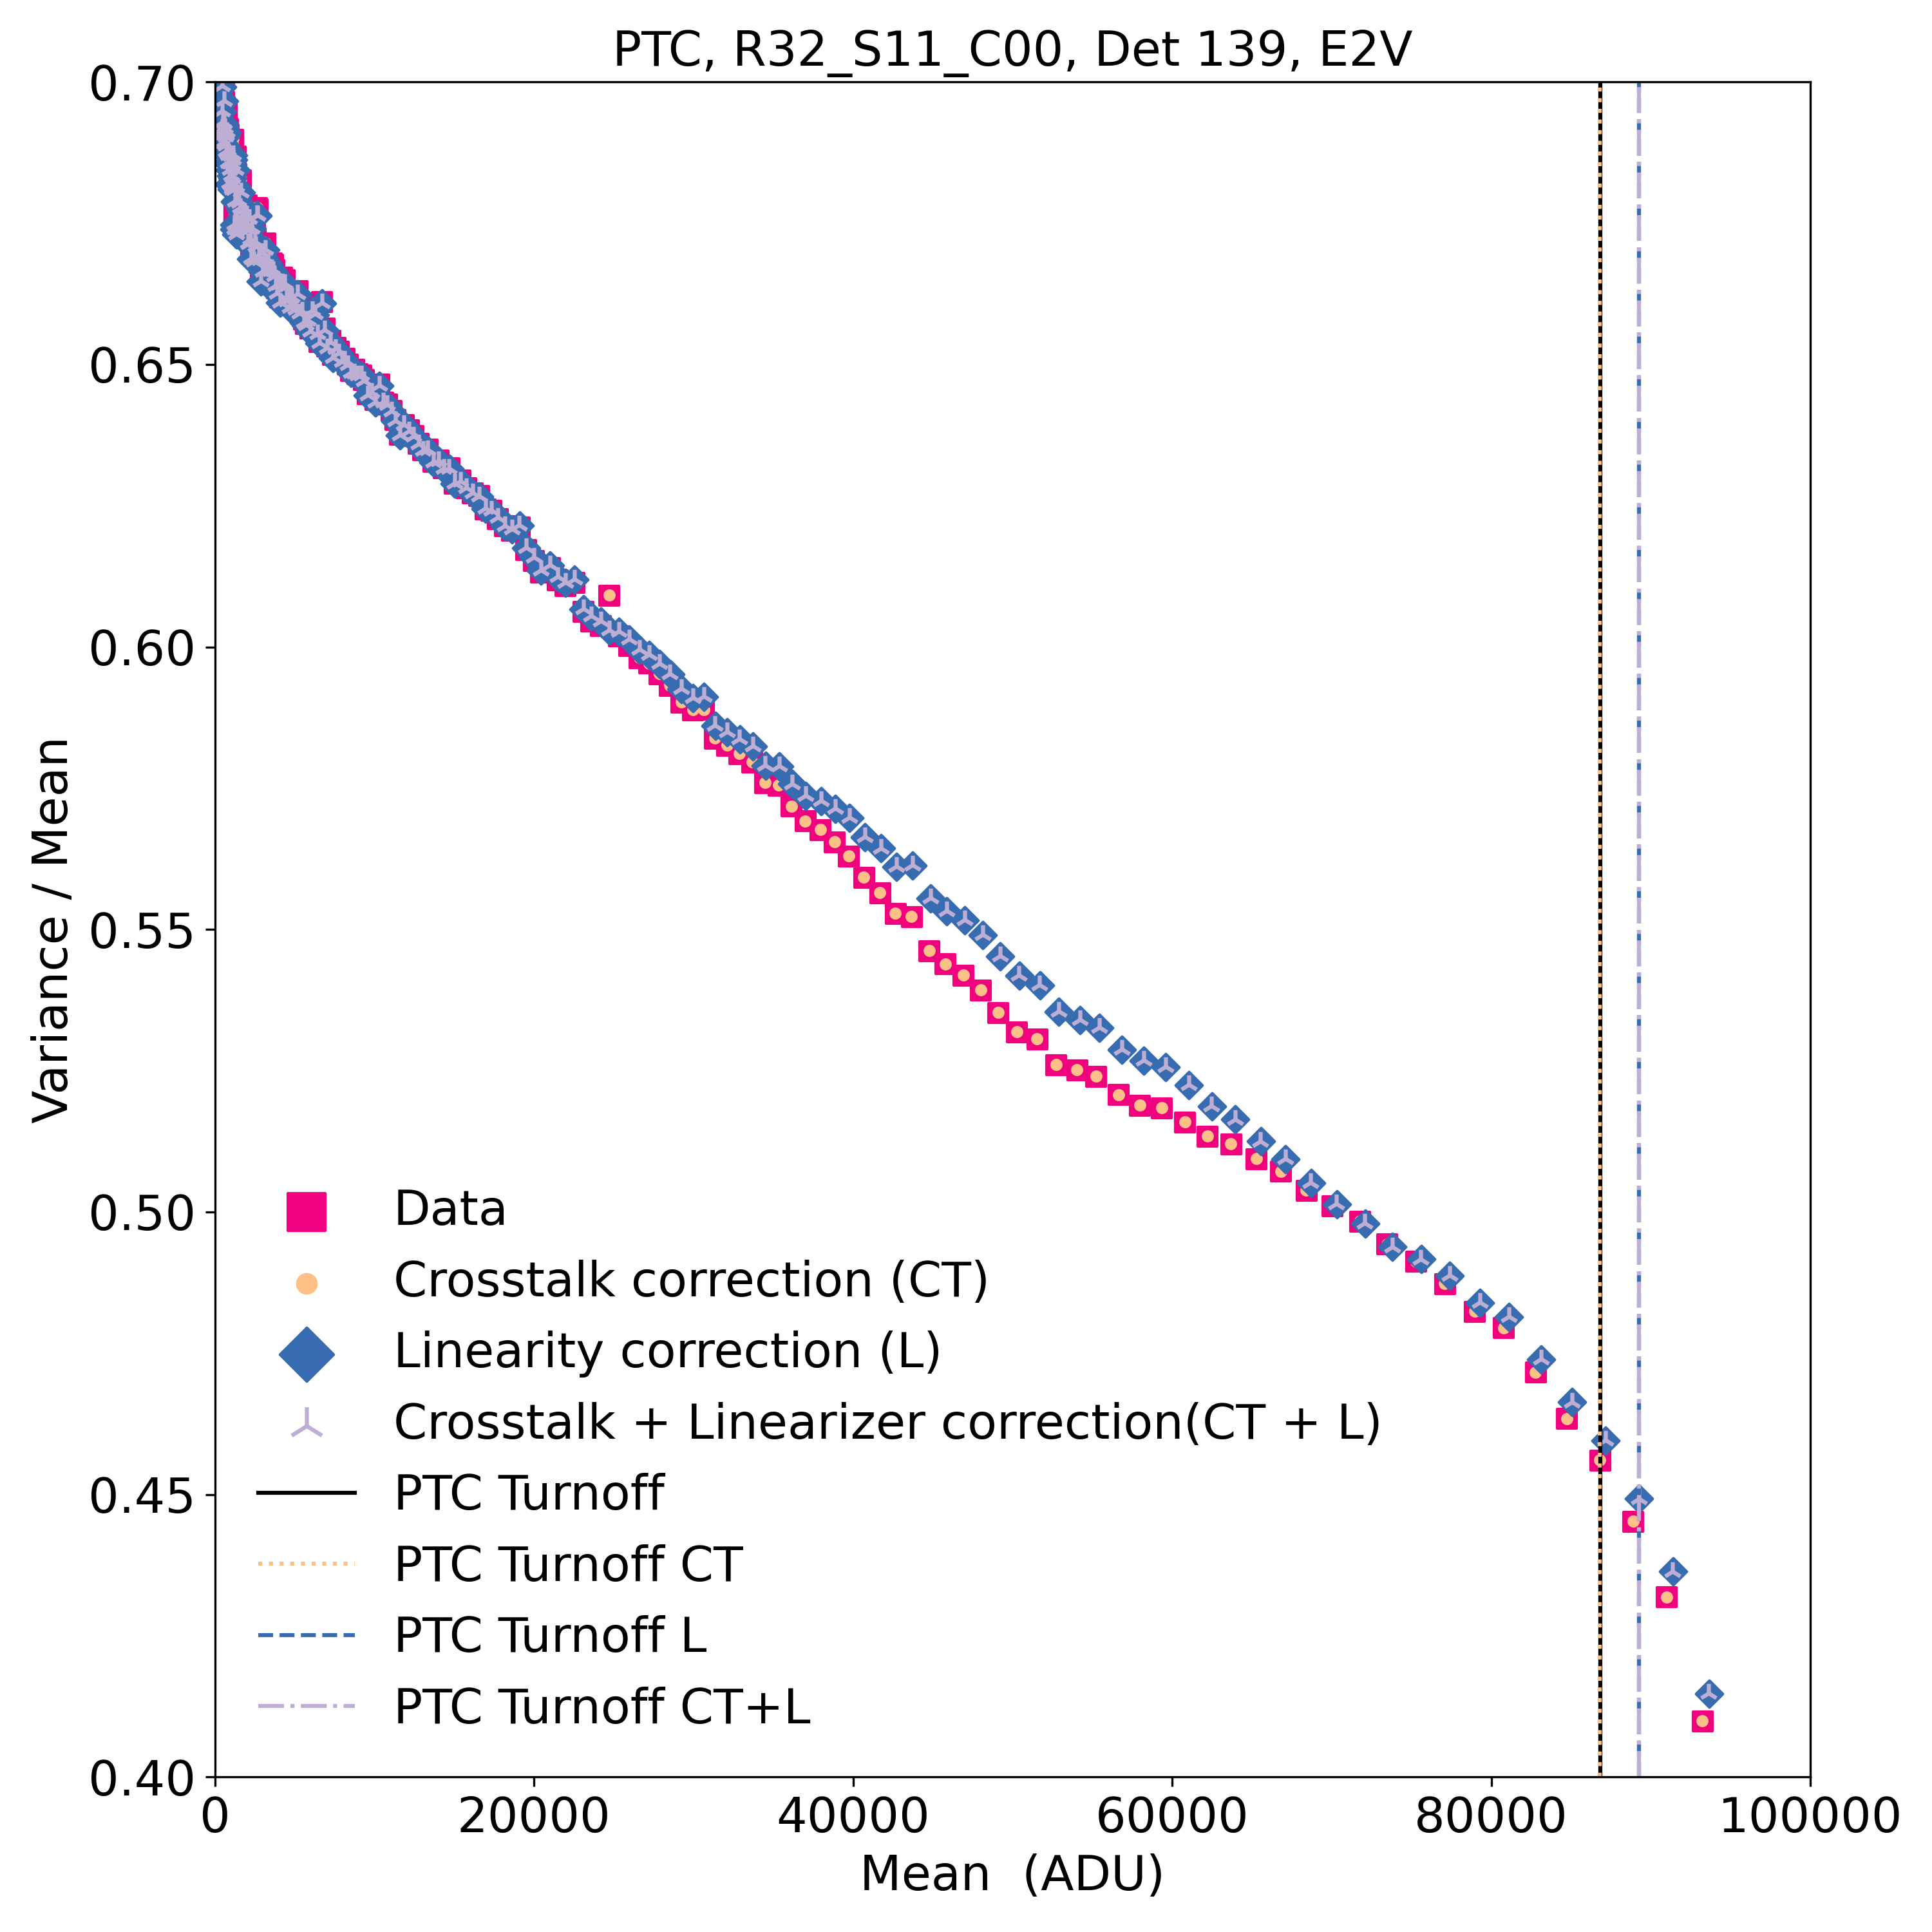
\includegraphics[width=\textwidth]{Figures/Variance_Mean_vs_Mean139.png}
     \end{subfigure}
        \caption{Variance normalized by mean vs. mean, for detector 32 (R10\_S12) for vendor ITL, on the left, and for detector 139 (R32\_S11) for vendor E2V, on the right. We show the data with no correction by crosstalk (CT) and nonlinearity in magenta squares. The orange dots show the data corrected for CT. The data corrected for nonlinearity with blue diamonds. Also, the triangles for data with corrections by both effects: TC and nonlinearity. Finally, the vertical lines represent the location of the turnoff.}
        
        %Varianza normalizada por la media vs la media, del detector 32 (R10\_S12) para el fabricante ITL, a la izquierda, y para el detector 139 (R32\_S11) del fabricante E2V, a la derecha. Se muestra en cuadrados magenta los datos sin corregir por crosstalk (CT) o por la no linealidad, en punto naranja los datos corregidos por CT, por lo diamantes azules los datos corregidos por la no linealidad y por los triángulos los datos corregidos por estos dos efectos: CT y no linealidad. Las líneas verticales representan la ubicación del turnoff.}
        \label{fig:varmean_crosstalk}
\end{figure}


\cite{scipy_2020}